        %%******************************************%%
        %%                                          %%
        %%        Modello di tesi di laurea         %%
        %%            di Andrea Giraldin            %%
        %%                                          %%
        %%             2 novembre 2012              %%
        %%                                          %%
        %%******************************************%%


% I seguenti commenti speciali impostano:
% 1. 
% 2. PDFLaTeX come motore di composizione;
% 3. tesi.tex come documento principale;
% 4. il controllo ortografico italiano per l'editor.

% !TEX encoding = UTF-8
% !TEX TS-program = pdflatex
% !TEX root = tesi.tex
% !TEX spellcheck = it-IT

\documentclass[10pt,                    % corpo del font principale
               a4paper,                 % carta A4
               twoside,                 % impagina per fronte-retro
               openright,               % inizio capitoli a destra
               english,                 
               italian,                 
               ]{book}    

\usepackage[utf8]{inputenc}             % codifica di input; anche [latin1] va bene
                                        % NOTA BENE! va accordata con le preferenze dell'editor

%**************************************************************
% Importazione package
%************************************************************** 

%\usepackage{amsmath,amssymb,amsthm}    % matematica

\usepackage[english, italian]{babel}    % per scrivere in italiano e in inglese;
                                        % l'ultima lingua (l'italiano) risulta predefinita

\usepackage{bookmark}                   % segnalibri

\usepackage{caption}                    % didascalie

\usepackage{chngpage,calc}              % centra il frontespizio

\usepackage{csquotes}                   % gestisce automaticamente i caratteri (")

\usepackage{emptypage}                  % pagine vuote senza testatina e piede di pagina

\usepackage{epigraph}					% per epigrafi

\usepackage{eurosym}                    % simbolo dell'euro

\usepackage[T1]{fontenc}                % codifica dei font:
                                        % NOTA BENE! richiede una distribuzione *completa* di LaTeX

%\usepackage{indentfirst}               % rientra il primo paragrafo di ogni sezione

\usepackage{graphicx}                   % immagini

\usepackage{hyperref}                   % collegamenti ipertestuali



\usepackage[binding=5mm]{layaureo}      % margini ottimizzati per l'A4; rilegatura di 5 mm


\usepackage{listings}                   % codici

\usepackage{microtype}                  % microtipografia

\usepackage{mparhack,fixltx2e,relsize}  % finezze tipografiche

\usepackage{nameref}                    % visualizza nome dei riferimenti                                      

\usepackage[font=small]{quoting}        % citazioni

\usepackage{subfig}                     % sottofigure, sottotabelle

\usepackage[italian]{varioref}          % riferimenti completi della pagina

\usepackage[dvipsnames]{xcolor}         % colori

\usepackage{forest}

\usepackage{booktabs}                   % tabelle                                       
\usepackage{tabularx}                   % tabelle di larghezza prefissata                                    
\usepackage{longtable}                  % tabelle su più pagine                                        
\usepackage{ltxtable}                   % tabelle su più pagine e adattabili in larghezza

\usepackage[toc, acronym]{glossaries}   % glossario
                                        % per includerlo nel documento bisogna:
                                        % 1. compilare una prima volta tesi.tex;
                                        % 2. eseguire: makeindex -s tesi.ist -t tesi.glg -o tesi.gls tesi.glo
                                        % 3. eseguire: makeindex -s tesi.ist -t tesi.alg -o tesi.acr tesi.acn
                                        % 4. compilare due volte tesi.tex.

\usepackage[backend=biber,style=verbose-ibid,hyperref,backref]{biblatex}
                                        % eccellente pacchetto per la bibliografia; 
                                        % produce uno stile di citazione autore-anno; 
                                        % lo stile "numeric-comp" produce riferimenti numerici
                                        % per includerlo nel documento bisogna:
                                        % 1. compilare una prima volta tesi.tex;
                                        % 2. eseguire: biber tesi
                                        % 3. compilare ancora tesi.tex.

%**************************************************************
% file contenente le impostazioni della tesi
%**************************************************************

%**************************************************************
% Frontespizio
%**************************************************************
\newcommand{\myName}{Giovanni Mazzocchin}                                    % autore
\newcommand{\myTitle}{Analisi ed implementazione di un front-end per la lingua italiana all'interno
del motore di sintesi vocale Speect}                    
\newcommand{\myDegree}{Tesi di laurea triennale}                % tipo di tesi
\newcommand{\myUni}{Università degli Studi di Padova}           % università
\newcommand{\myFaculty}{Corso di Laurea in Informatica}         % facoltà
\newcommand{\myDepartment}{Dipartimento di Matematica}          % dipartimento
\newcommand{\myProf}{Paolo Baldan}                                % relatore
\newcommand{\myLocation}{Padova}                                % dove
\newcommand{\myAA}{2015-2016}                                   % anno accademico
\newcommand{\myTime}{Agosto 2016}                                  % quando


%**************************************************************
% Impostazioni di impaginazione
% see: http://wwwcdf.pd.infn.it/AppuntiLinux/a2547.htm
%**************************************************************

\setlength{\parindent}{14pt}   % larghezza rientro della prima riga
\setlength{\parskip}{0pt}   % distanza tra i paragrafi


%**************************************************************
% Impostazioni di biblatex
%**************************************************************
\bibliography{bibliografia} % database di biblatex 

\defbibheading{bibliography}
{
    \cleardoublepage
    \phantomsection 
    \addcontentsline{toc}{chapter}{\bibname}
    \chapter*{\bibname\markboth{\bibname}{\bibname}}
}

\setlength\bibitemsep{1.5\itemsep} % spazio tra entry

\DeclareBibliographyCategory{opere}
\DeclareBibliographyCategory{web}

\addtocategory{opere}{womak:lean-thinking}
\addtocategory{web}{site:agile-manifesto}

\defbibheading{opere}{\section*{Riferimenti bibliografici}}
\defbibheading{web}{\section*{Siti Web consultati}}


%**************************************************************
% Impostazioni di caption
%**************************************************************
\captionsetup{
    tableposition=top,
    figureposition=bottom,
    font=small,
    format=hang,
    labelfont=bf
}

%**************************************************************
% Impostazioni di glossaries
%**************************************************************
% !TEX encoding = UTF-8
% !TEX TS-program = pdflatex
% !TEX root = ../tesi.tex
% !TEX spellcheck = it-IT

%**************************************************************
% Bibliografia
%**************************************************************

\cleardoublepage
\chapter{Glossario}

\paragraph{binutils}
  formalmente \textit{GNU Binutils}, è un insieme di \textit{tool} binari per \textit{GNU}, comprendente, fra
  gli altri, i programmi \texttt{ld} (\textit{GNU linker}) e \texttt{as} (\textit{GNU assembler}).
\label{glo:binu}


\paragraph{consonante approssimante}
\label{glo:consappr}
   classe di suoni che comprende le \textit{semivocali} o \textit{semiconsonanti}, ossia suoni che
   si trovano al confine tra l'articolazione consonantica e quella vocalica.

\paragraph{consonante fricativa}
\label{glo:consfric}
   classe di suoni prodotti mediante un restringimento tra alcuni organi nella cavità orale, che si avvicinano
   senza chiudersi totalmente come avviene per le consonanti occlusive.

\paragraph{consonante laterale}
\label{glo:conslate}
   classe di suoni prodotti mediante una parziale occlusione del canale orale, provocata dalla lingua che
   ne ostruisce la parte centrale lasciando spazio solo ai lati.

\paragraph{consonante nasale}
\label{glo:consnasa}
  classe di suoni caratterizzata da una risonanza che si realizza quando il canale orale viene ostruito, mentre il velo
  palatino rimane abbassato, permettendo il deflusso dell'aria proveniente dai polmoni e dalle fosse nasali.

\paragraph{consonante occlusiva}
\label{glo:consoccl}
  classe di suoni generati mediante il blocco completo del flusso di aria a livello della bocca,
  della faringe e della glottide.
\paragraph{consonante sorda}
\label{glo:conssord}
  classe di suoni articolati senza la vibrazione delle corde vocali.

\paragraph{consonante vibrante}
\label{glo:consvibr}
  classe di suoni prodotti mediante una debole occlusione intermittente del canale orale, la quale
  si interrompe e ripristina velocemente più volte.

\paragraph{hot swapping} 
\label{glo:hots}
 detto anche \textit{hot plugging}, è la capacità di un sistema di sostituire e caricare componenti
 senza la necessità di un suo spegnimento.

\paragraph{OCaml}
\label{glo:ocam}
  ossia \textit{Objective-Caml}, è la principale implementazione del linguaggio \textit{Caml}.

\paragraph{XSL}
\label{glo:xsl}
  sigla di \textit{e\textbf{X}tensible \textbf{S}tylesheet \textbf{L}anguage}, è il linguaggio di descrizione
  dei fogli di stile per i documenti in formato \textit{XML}.


\paragraph{POS tagging}
\label{glo:postag}
  noto anche come \textit{grammatical tagging} o \textit{word-category disambiguation}, è il processo che si occupa
  dell'associazione di una parte del discorso a ciascuna parola in una frase.
 % database di termini
\makeglossaries


%**************************************************************
% Impostazioni di graphicx
%**************************************************************
\graphicspath{{immagini/}} % cartella dove sono riposte le immagini


%**************************************************************
% Impostazioni di hyperref
%**************************************************************
\hypersetup{
    %hyperfootnotes=false,
    %pdfpagelabels,
    %draft,	% = elimina tutti i link (utile per stampe in bianco e nero)
    colorlinks=true,
    linktocpage=true,
    pdfstartpage=1,
    pdfstartview=FitV,
    % decommenta la riga seguente per avere link in nero (per esempio per la stampa in bianco e nero)
    %colorlinks=false, linktocpage=false, pdfborder={0 0 0}, pdfstartpage=1, pdfstartview=FitV,
    breaklinks=true,
    pdfpagemode=UseNone,
    pageanchor=true,
    pdfpagemode=UseOutlines,
    plainpages=false,
    bookmarksnumbered,
    bookmarksopen=true,
    bookmarksopenlevel=1,
    hypertexnames=true,
    pdfhighlight=/O,
    %nesting=true,
    %frenchlinks,
    urlcolor=webbrown,
    linkcolor=RoyalBlue,
    citecolor=webgreen,
    %pagecolor=RoyalBlue,
    %urlcolor=Black, linkcolor=Black, citecolor=Black, %pagecolor=Black,
    pdftitle={\myTitle},
    pdfauthor={\textcopyright\ \myName, \myUni, \myFaculty},
    pdfsubject={},
    pdfkeywords={},
    pdfcreator={pdfLaTeX},
    pdfproducer={LaTeX}
}

%**************************************************************
% Impostazioni di itemize
%**************************************************************
\renewcommand{\labelitemi}{$\ast$}

%\renewcommand{\labelitemi}{$\bullet$}
%\renewcommand{\labelitemii}{$\cdot$}
%\renewcommand{\labelitemiii}{$\diamond$}
%\renewcommand{\labelitemiv}{$\ast$}


%**************************************************************
% Impostazioni di listings
%**************************************************************
\lstset{
    language=[LaTeX]Tex,%C++,
    keywordstyle=\color{RoyalBlue}, %\bfseries,
    basicstyle=\small\ttfamily,
    %identifierstyle=\color{NavyBlue},
    commentstyle=\color{Green}\ttfamily,
    stringstyle=\rmfamily,
    numbers=none, %left,%
    numberstyle=\scriptsize, %\tiny
    stepnumber=5,
    numbersep=8pt,
    showstringspaces=false,
    breaklines=true,
    frameround=ftff,
    frame=single
} 


%**************************************************************
% Impostazioni di xcolor
%**************************************************************
\definecolor{webgreen}{rgb}{0,.5,0}
\definecolor{webbrown}{rgb}{.6,0,0}


%**************************************************************
% Altro
%**************************************************************

\newcommand{\omissis}{[\dots\negthinspace]} % produce [...]

% eccezioni all'algoritmo di sillabazione
\hyphenation
{
    ma-cro-istru-zio-ne
    gi-ral-din
}

\newcommand{\sectionname}{sezione}
\addto\captionsitalian{\renewcommand{\figurename}{figura}
                       \renewcommand{\tablename}{tabella}}

\newcommand{\glsfirstoccur}{\ap{{[g]}}}

\newcommand{\intro}[1]{\emph{\textsf{#1}}}

%**************************************************************
% Environment per ``rischi''
%**************************************************************
\newcounter{riskcounter}                % define a counter
\setcounter{riskcounter}{0}             % set the counter to some initial value

%%%% Parameters
% #1: Title
\newenvironment{risk}[1]{
    \refstepcounter{riskcounter}        % increment counter
    \par \noindent                      % start new paragraph
    \textbf{\arabic{riskcounter}. #1}   % display the title before the 
                                        % content of the environment is displayed 
}{
    \par\medskip
}

\newcommand{\riskname}{Rischio}

\newcommand{\riskdescription}[1]{\textbf{\\Descrizione:} #1.}

\newcommand{\risksolution}[1]{\textbf{\\Soluzione:} #1.}

%**************************************************************
% Environment per ``use case''
%**************************************************************
\newcounter{usecasecounter}             % define a counter
\setcounter{usecasecounter}{0}          % set the counter to some initial value

%%%% Parameters
% #1: ID
% #2: Nome
\newenvironment{usecase}[2]{
    \renewcommand{\theusecasecounter}{\usecasename #1}  % this is where the display of 
                                                        % the counter is overwritten/modified
    \refstepcounter{usecasecounter}             % increment counter
    \vspace{10pt}
    \par \noindent                              % start new paragraph
    {\large \textbf{\usecasename #1: #2}}       % display the title before the 
                                                % content of the environment is displayed 
    \medskip
}{
    \medskip
}

\newcommand{\usecasename}{UC}

\newcommand{\usecaseactors}[1]{\textbf{\\Attori Principali:} #1. \vspace{4pt}}
\newcommand{\usecasepre}[1]{\textbf{\\Precondizioni:} #1. \vspace{4pt}}
\newcommand{\usecasedesc}[1]{\textbf{\\Descrizione:} #1. \vspace{4pt}}
\newcommand{\usecasepost}[1]{\textbf{\\Postcondizioni:} #1. \vspace{4pt}}
\newcommand{\usecasealt}[1]{\textbf{\\Scenario Alternativo:} #1. \vspace{4pt}}

%**************************************************************
% Environment per ``namespace description''
%**************************************************************

\newenvironment{namespacedesc}{
    \vspace{10pt}
    \par \noindent                              % start new paragraph
    \begin{description} 
}{
    \end{description}
    \medskip
}

\newcommand{\classdesc}[2]{\item[\textbf{#1:}] #2}
                     % file con le impostazioni personali  INPUT o INCLUDE?

\begin{document}
%**************************************************************
% Materiale iniziale
%**************************************************************
\frontmatter
% !TEX encoding = UTF-8
% !TEX TS-program = pdflatex
% !TEX root = ../tesi.tex
% !TEX spellcheck = it-IT

%**************************************************************
% Frontespizio 
%**************************************************************
\begin{titlepage}

\begin{center}

\begin{LARGE}
\textbf{\myUni}\\
\end{LARGE}

\vspace{10pt}

\begin{Large}
\textsc{\myDepartment}\\
\end{Large}

\vspace{10pt}

\begin{large}
\textsc{\myFaculty}\\
\end{large}

\vspace{30pt}
\begin{figure}[htbp]
\begin{center}

\includegraphics[height=6cm]{logo-unipd}
\end{center}
\end{figure}
\vspace{30pt} 

\begin{LARGE}
\begin{center}
\textbf{\myTitle}\\
\end{center}
\end{LARGE}

\vspace{10pt} 

\begin{large}
\textsl{\myDegree}\\
\end{large}

\vspace{40pt} 

\begin{large}
\begin{flushleft}
\textit{Relatore}\\ 
\vspace{5pt} 
Prof. \myProf
\end{flushleft}

\vspace{0pt} 

\begin{flushright}
\textit{Laureando}\\ 
\vspace{5pt} 
\myName
\end{flushright}
\end{large}

\vspace{40pt}

\line(1, 0){338} \\
\begin{normalsize}
\textsc{Anno Accademico \myAA}
\end{normalsize}

\end{center}
\end{titlepage} 
% !TEX encoding = UTF-8
% !TEX TS-program = pdflatex
% !TEX root = ../tesi.tex
% !TEX spellcheck = it-IT

%**************************************************************
% Colophon
%**************************************************************
\clearpage
\phantomsection
\thispagestyle{empty}

\hfill

\vfill

\noindent\myName: \textit{\myTitle,}
\myDegree,
\textcopyright\ \myTime.
%% !TEX encoding = UTF-8
% !TEX TS-program = pdflatex
% !TEX root = ../tesi.tex
% !TEX spellcheck = it-IT

%**************************************************************
% Dedica
%**************************************************************
\cleardoublepage
\phantomsection
\thispagestyle{empty}
\pdfbookmark{Dedica}{Dedica}

\vspace*{3cm}

\begin{center}
Lorem ipsum dolor sit amet, consectetuer adipiscing elit. \\ \medskip
--- Oscar Wilde    
\end{center}

\medskip

\begin{center}
Dedicato a ...
\end{center}

% !TEX encoding = UTF-8
% !TEX TS-program = pdflatex
% !TEX root = ../tesi.tex
% !TEX spellcheck = it-IT

%**************************************************************
% Sommario
%**************************************************************
\cleardoublepage
\phantomsection
\pdfbookmark{Sommario}{Sommario}
\begingroup
\let\clearpage\relax
\let\cleardoublepage\relax
\let\cleardoublepage\relax

\chapter*{Sommario}

Il presente documento descrive il lavoro svolto durante l'attività di \textit{stage}, della durata di circa trecentoventi ore, dal laureando Giovanni Mazzocchin presso l'azienda Mivoq S.r.L. \\ Il progetto sviluppato in questo \textit{stage} si inquadra in un’attività di medio/lungo
termine che consiste nella migrazione del motore di sintesi utilizzato dall’azienda 
da una piattaforma \textit{Java} (\textbf{MaryTTS}) ad una \textit{C} (\textbf{Speect}).

%\vfill
%
%\selectlanguage{english}
%\pdfbookmark{Abstract}{Abstract}
%\chapter*{Abstract}
%
%\selectlanguage{italian}

\endgroup			

\vfill


% !TEX encoding = UTF-8
% !TEX TS-program = pdflatex
% !TEX root = ../tesi.tex
% !TEX spellcheck = it-IT

%**************************************************************
% Ringraziamenti
%**************************************************************
\cleardoublepage
\phantomsection
\pdfbookmark{Ringraziamenti}{ringraziamenti}

%\begin{flushright}{
%	\slshape    
%	``Life is really simple, but we insist on making it complicated''} \\ 
%	\medskip
 %   --- Confucius
%\end{flushright}


\bigskip

\begingroup
\let\clearpage\relax
\let\cleardoublepage\relax
\let\cleardoublepage\relax

\chapter*{Ringraziamenti}

\noindent \textit{Innanzitutto, vorrei esprimere la mia gratitudine al Prof. Paolo Baldan, relatore della mia tesi, per l'aiuto e il sostegno fornitomi durante la stesura del lavoro.}\\

\noindent \textit{Desidero ringraziare con affetto i miei genitori per il sostegno, il grande aiuto e per essermi stati vicini in ogni momento durante gli anni di studio.}\\

\bigskip

\noindent\textit{\myLocation, \myTime}
\hfill \myName

\endgroup


% !TEX encoding = UTF-8
% !TEX TS-program = pdflatex
% !TEX root = ../tesi.tex
% !TEX spellcheck = it-IT

%**************************************************************
% Indici
%**************************************************************
\cleardoublepage
\pdfbookmark{\contentsname}{tableofcontents}
\setcounter{tocdepth}{2}
\tableofcontents
%\markboth{\contentsname}{\contentsname} 
\clearpage

\begingroup 
    \let\clearpage\relax
    \let\cleardoublepage\relax
    \let\cleardoublepage\relax
    %*******************************************************
    % Elenco delle figure
    %*******************************************************    
    \phantomsection
    \pdfbookmark{\listfigurename}{lof}
    \listoffigures

    \vspace*{8ex}

    %*******************************************************
    % Elenco delle tabelle
    %*******************************************************
    \phantomsection
    \pdfbookmark{\listtablename}{lot}
    \listoftables
        
    \vspace*{8ex}
\endgroup

\cleardoublepage

\cleardoublepage

%**************************************************************
% Materiale principale
%**************************************************************
\mainmatter
% !TEX encoding = UTF-8
% !TEX TS-program = pdflatex
% !TEX root = ../tesi.tex
% !TEX spellcheck = it-IT

%**************************************************************
\chapter{Introduzione}
\label{cap:introduzione}
%**************************************************************

%Introduzione al contesto applicativo.\\

%\noindent Esempio di utilizzo di un termine nel glossario \\
%\gls{api}. \\

%\noindent Esempio di citazione in linea \\
%\cite{site:agile-manifesto}. \\

%\noindent Esempio di citazione nel pie' di pagina \\
%citazione\footcite{womak:lean-thinking} \\

%**************************************************************
\section{L'azienda e lo stage}

\href{https://www.mivoq.it/}{Mivoq S.r.L.} è un'azienda operante nel settore delle tecnologie vocali, nata nel 2013 come
\textit{spinoff} dell'\href{http://www.istc.cnr.it/it}{Istituto di Scienze e Tecnologie della Cognizione} del 
\href{https://www.cnr.it/}{Consiglio Nazionale delle Ricerche}. L'azienda propone l'utilizzo delle tecnologie vocali per permettere a chiunque di creare e personalizzare la propria voce sintetica in breve tempo. \\

%**************************************************************
Lo \textit{stage} ha avuto una durata di due mesi per un totale di 320 ore, da maggio 2016 a luglio 2016.
La politica aziendale non adotta orari fissi per i propri dipendenti, tuttavia ho sempre cercato di lavorare
7-8 ore al giorno dal lunedì al venerdì per non superare i due mesi di tirocinio. \\ Ho avuto la possibilità di
lavorare  sia nelle due sedi di Mivoq (Padova e Bassano del Grappa) sia a casa, ma in costante contatto
con il \textit{tutor} aziendale Giulio Paci. \\ Sia io sia il \textit{tutor} abbiamo mantenuto costantemente aggiornati dei \textit{report}
contenenti i \textit{task} assegnati e la descrizione del progresso nel loro svolgimento. 

\begin{figure}[!h] 
    		\centering 
    		
\includegraphics[width=0.5\columnwidth]{mivoq-logo} 
   	 	\caption{Logo dell'azienda}
\end{figure}

\section{Descrizione generale di Speect e idea complessiva del progetto}
\textbf{Speect} è una piattaforma di \textit{Text to Speech (TTS)} multilingua sviluppata dal gruppo 
\href{http://www.meraka.org.za/humanLanguage.htm}{Human Language Technologies}
del \href{http://www.csir.co.za/meraka/}{Meraka Institute}, in Sudafrica. \\ Le componenti base del sistema sono implementate in linguaggio \textit{C}, rispettando
rigidamente le direttive dello \textit{standard} \href{http://www.dii.uchile.cl/~daespino/files/Iso_C_1999_definition.pdf}{ISO/IEC 9899:1990}; 
\textbf{Speect} inoltre implementa il paradigma ad oggetti ed è \textit{multithreading}. \\ Il sistema è stato progettato in modo da essere facilmente estensibile
tramite \textit{plug-in}: in particolare, tutti i processi di sintesi (dal \textit{Tokenizer} al \textit{Vocoder}, passando per il \textit{Phonemizer}) 
sono implementati come \textit{plug-in}. \\ L'\textit{engine} di \textbf{Speect}
si occupa invece della definizione dei tipi astratti e della comunicazione tra i vari \textit{plug-in}; esso implementa
inoltre la struttura dati principale di \textbf{Speect}, l'\textit{Heterogeneous Relation Graph}, struttura continuamente
modificata ed estesa dai \textit{plug-in} in esecuzione. \\
Il \textit{plug-in} che si occupa del \hyperref[glo:postag]{\emph{Pos tagging}\glsfirstoccur} all'interno di \textbf{Speect}
è un \textit{wrapper} di \href{https://github.com/mivoq/hunpos}{Hunpos} (al quale hanno lavorato i due tirocinanti
precedenti), un'implementazione \textit{open source} di un algoritmo
che utilizza il \href{https://en.wikipedia.org/wiki/Hidden_Markov_model}{Modello di Markov Nascosto}; \textit{Hunpos} è una 
reimplementazione in linguaggio \hyperref[glo:ocam]{\emph{OCaml}\glsfirstoccur} di 
\href{http://www.coli.uni-saarland.de/~thorsten/tnt/}{TnT}, un \textit{part-of-speech tagger} sviluppato da Thorsten Brants. \\

Il progetto sviluppato in questo \textit{stage} si inquadra in un'attività di medio/lungo termine che consiste nella migrazione 
del motore di sintesi utilizzato dall'azienda da una piattaforma \textit{Java} (\textbf{MaryTTS}) ad una \textit{C} (\textbf{Speect}). \\
\textbf{MaryTTS} è un sistema scritto in \textit{Java}, fornisce dei buoni strumenti per l'analisi interna, tuttavia presenta i seguenti difetti:
   \begin{itemize}
        \item basse \textit{performance} dovute al linguaggio; 
        \item molto codice duplicato e troppe dipendenze; 
        \item struttura ad albero rigida per contenere le informazioni ricavate dal \textit{front-end}: ciò rende complicato
              realizzare alcune analisi linguistiche;
        \item difficoltà nel modificare il \textit{vocoder} mantenendo la compatibilità all'indietro;
        \item carenza di librerie adeguate per \textit{Java} per effettuare il processamento audio;
        \item struttura modulare rigida per le lingue e le voci;
        \item \textit{iOS} non supporta \textit{Java}, e in futuro potrebbe essere interesse dell'azienda sviluppare per questa piattaforma.
   \end{itemize}
L'azienda prevede dunque di poter estendere \textbf{Speect} fino al momento in cui esso conterrà un sottoinsieme delle funzionalità
di \textbf{MaryTTS}, con lo scopo di utilizzarlo come sistema di \textit{TTS} nei servizi e nei prodotti forniti da Mivoq. \\
L'attività primaria dello \textit{stage} è stata dunque l'implementazione di alcuni passaggi di tale migrazione, tra cui il miglioramento
di una voce sintetica in lingua italiana tramite l'estensione e la creazione di alcuni \textit{plug-in}. \\
I due tirocinanti precedenti avevano sviluppato le componenti \textit{Tokenizer}, \textit{POS tagger} e \textit{trascrittore fonetico};
inoltre essi avevano lavorato ad una \textit{suite} di \textit{tool} (principalmente \textit{script bash} e fogli \hyperref[glo:xsl]{\emph{XSL}\glsfirstoccur}) 
per agevolare il confronto tra i due sistemi \textbf{MaryTTS} e \textbf{Speect}, \textit{suite} alla quale ho lavorato anche io per un
 breve periodo (circa tre giorni) all'inizio dello \textit{stage} come introduzione al sistema. \\
Prima del mio \textit{stage} la qualità della voce sintetica italiana era piuttosto bassa, principalmente a causa
dei seguenti motivi:
 \begin{itemize}
   \item il testo in lingua italiana veniva sillabificato secondo le regole della lingua inglese
         in quanto mancava il \textit{plug-in} specifico per l'italiano adatto a questo scopo;
   \item molte \textit{feature} utili alla produzione dell'audio da parte del \textit{vocoder} non venivano calcolate
         o raccolte propriamente, fornendo così al \textit{back-end} un numero insufficiente di informazioni sull'\textit{input}.
 \end{itemize}
Per quanto riguarda il metodo adottato nello sviluppo del progetto, l'assenza di documentazione (se non nei commenti al codice) 
riguardante i \textit{plug-in} sviluppati dai tirocinanti precedenti (sui quali ho lavorato) ha reso necessari uno studio continuo del 
codice sorgente e l'esecuzione di numerosi \textit{test} per comprendere il funzionamento del sistema. \\ 
Ad ogni modo, in alcuni casi, l'interazione con il \textit{tutor} aziendale è stata
indispensabile e fondamentale per la comprensione dei dettagli più ostici.


%*************************************
\section{Problematiche riscontrate}
 \subsection{Documentazione di Speect}
  La documentazione di \textbf{Speect} è piuttosto scarsa e contiene alcuni errori che possono confondere il principiante, inoltre
  gli sviluppatori originali hanno abbandonato il progetto nel 2013, pertanto non esistono aggiornamenti alla documentazione da molto tempo.
  Inoltre, effettuando delle ricerche tramite i principali \textit{search engine}, sembra evidente come \textbf{Speect} non abbia ricevuto molta attenzione
  al di fuori dell'istituto nel quale è stato sviluppato (oltre a Mivoq ovviamente). \\ Pertanto non è stato possibile nemmeno 
  rivolgersi a \textit{forum} o fonti di terze parti per la risoluzione di problemi anche banali (la tipica ricerca su 
  \textit{Google} non restituiva risultati specifici). Per questo motivo la risoluzione di problemi anche banali
  ha richiesto un numero di ore non irrilevante. \\
  È inoltre notevole il fatto che la mancanza/scarsa qualità di documentazione a volte abbia reso necessaria l'analisi del codice sorgente 
  interno all'\textit{engine} di \textbf{Speect}. \\
  Visti i problemi citati sopra, nel corso dello \textit{stage} è stato ritenuto opportuno stilare una lista 
  (condivisa con il \textit{tutor} aziendale) degli errori individuati nella documentazione.
  
%*************************************
\section{Prodotto ottenuto}
Tutto il lavoro svolto durante lo \textit{stage} è rientrato nel percorso tracciato dai due tirocinanti
precedenti, i quali hanno sviluppato parte di un \textit{front-end} minimale per la lingua italiana per \textbf{Speect}.
Il mio compito è stato dunque lo sviluppo di nuove funzionalità per tale \textit{front-end} allo scopo di 
renderlo più maturo, ottenendo una voce in lingua italiana di qualità superiore.\\
In particolare, le (macro)attività svolte durante il tirocinio sono state le seguenti:
    \begin{itemize} 
       \item miglioramento del \textit{plug-in} responsabile della scrittura in formato \textit{MaryXML}
             dei dati interni all'\textit{HRG} di \textbf{Speect}; sono inoltre stati estesi i \textit{test} esistenti
             per verificare il comportamento del \textit{plug-in} dopo le estensioni;
       \item sviluppo di un sillabificatore completo per l'italiano e dei \textit{test} per 
             verificarne il corretto funzionamento su un grande numero di possibili \textit{input};
       \item analisi ed implementazione di alcune componenti per il calcolo 
             delle \textit{feature} utili per il \textit{vocoder} (è stato cioè migliorato il passaggio
             dei dati dal \textit{front-end} al \textit{back-end}). \\
    \end{itemize}
Dopo il termine del mio \textit{stage} l'azienda procederà con lo sviluppo di \textbf{Speect}, avendo come obiettivo
un prodotto dotato di tutte le funzionalità di \textbf{MaryTTS} e in grado di sostituirlo per l'utilizzo aziendale. 


%**************************************************************
\newpage
\section{Organizzazione del testo}

\begin{description}
    \item[{\hyperref[cap:analisi-requisiti]{Il secondo capitolo}}] presenta brevemente il sistema e descrive i requisiti del progetto;
    
    \item[{\hyperref[cap:speect]{Il terzo capitolo}}] descrive in profondità le componenti fondamentali del \textit{software} \textbf{Speect};
    
   % \item[{\hyperref[cap:analisi-requisiti]{Il quarto capitolo}}] approfondisce ...
    
    \item[{\hyperref[cap:progettazione-realizzazione]{Il quarto capitolo}}] descrive le scelte progettuali e di codifica, dal sillabificatore
      per l'italiano ai \textit{plug-in} per il calcolo delle \textit{feature};
    
    \item[{\hyperref[cap:verifica-validazione]{Il quinto capitolo}}] descrive le attività di verifica e validazione svolte sulle
      componenti prodotte durante lo \textit{stage};
    
    \item[{\hyperref[cap:conclusioni]{Il sesto capitolo}}] contiene alcune considerazioni finali sullo \textit{stage}.
\end{description}

Riguardo la stesura del testo, relativamente al documento sono state adottate le seguenti convenzioni tipografiche:
\begin{itemize}
	\item gli acronimi, le abbreviazioni e i termini ambigui o di uso non comune menzionati vengono definiti nel glossario, situato alla fine del presente documento;
	\item per le occorrenze dei termini riportati nel glossario viene utilizzata la seguente nomenclatura: \emph{parola}\glsfirstoccur;
	\item i termini in lingua straniera o facenti parti del gergo tecnico sono evidenziati con il carattere \emph{corsivo}.
\end{itemize}
             % Introduzione
% !TEX encoding = UTF-8
% !TEX TS-program = pdflatex
% !TEX root = ../tesi.tex
% !TEX spellcheck = it-IT

%**************************************************************
\chapter{Analisi dei Requisiti}
\label{cap:analisi-requisiti}
%**************************************************************

%\intro{Brevissima introduzione al capitolo}\\

%**************************************************************
\section{Descrizione di un generico sistema di sintesi vocale}
La \textbf{sintesi vocale} (in inglese \textit{speech synthesis}) è la tecnica per la riproduzione
artificiale della voce umana.\\ I sistemi di sintesi vocale (o sistemi \textbf{TTS}, dall'inglese \textit{Text To Speech})
 sono in genere composti da due parti interagenti ma operanti in ambiti differenti:
\begin{itemize}
  \item \textbf{front-end}: è la parte del sistema che si occupa della conversione del testo in \textit{input} in simboli fonetici 
                            interpretabili dal \textit{back-end};
  \item \textbf{back-end}: è la parte del sistema che interpreta e trasforma i simboli fonetici ricevuti in \textit{input} 
                           dal \textit{front-end}, producendo infine audio.
\end{itemize}
Il primo compito del \textit{front-end} è l'analisi del testo con lo scopo di espanderne i numeri, le sigle,
le date e le abbreviazioni in parole estese. \\
In una fase successiva le parole vengono convertite nelle trascrizioni fonetiche corrispondenti e viene
effettuata la suddivisione del testo in frasi e paragrafi. \\
I cinque processi del sistema nel suo complesso sono dunque:
\begin{itemize}
  \item \texttt{Tokenizer} (\textit{front-end}): processo che suddivide l'\textit{input} in \textit{utterance};
  \item \texttt{Espansione o normalizzazione} (\textit{front-end}): processo che espande o normalizza una \textit{utterance};
  \item \texttt{Phonemiser} (\textit{front-end}): processo che converte le parole nelle trascrizioni fonetiche corrispondenti;
  \item \texttt{Calcolo e raccolta delle feature} (\textit{front-end}): gruppo di processi che calcolano e aggiungono ulteriori
               informazioni alle \textit{utterance};
  \item \texttt{Vocoder} (\textit{back-end}): processo generatore dell'audio finale.
\end{itemize}

\begin{figure}[!h] 
    \centering 
    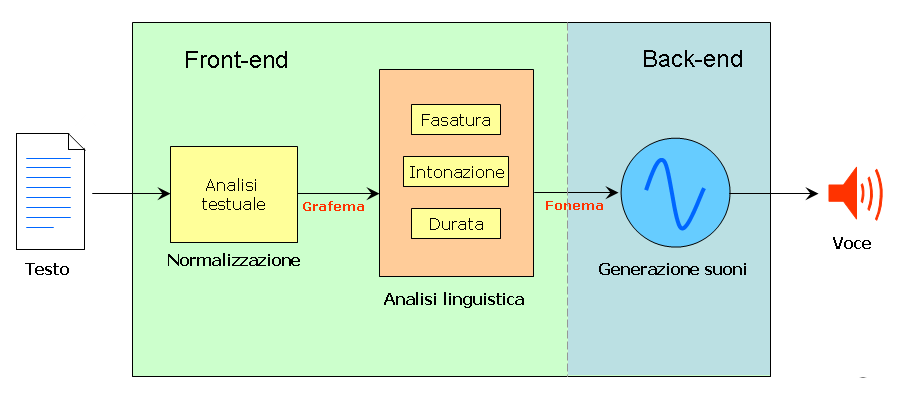
\includegraphics[width=0.9\columnwidth]{Sintesi_vocale} 
    \caption{Architettura di un sistema di \textbf{TTS}}
\end{figure}

\newpage

\section{Requisiti}
Di seguito viene riportata una lista esaustiva dei requisiti individuati all'inizio dell'attività di \textit{stage}.
Essi vengono classificati secondo i seguenti codici aggiunti in coda al carattere \textbf{R}:
%Da un'attenta analisi dei requisiti e degli use case effettuata sul progetto è stata stilata la tabella che traccia i requisiti in rapporto agli use case.\\
%Sono stati individuati diversi tipi di requisiti e si è quindi fatto utilizzo di un codice identificativo per distinguerli.\\
%Il codice dei requisiti è così strutturato R(F/Q/V)(N/D/O) dove:
\begin{enumerate}
    \item[\textbf{F} =] requisito funzionale;
    \item[\textbf{Q} =] requisito di qualità;
    \item[\textbf{V} =] requisito di vincolo;
    \item[\textbf{O} =] requisito obbligatorio;
    \item[\textbf{D} =] requisito desiderabile;
    \item[\textbf{Z} =] requisito opzionale.
\end{enumerate}
    %BEGIN of table
    %Tabella 
      \begin{center}
        \bgroup
        \def\arraystretch{1.8}
        \begin{longtable}{ | l | p{2cm} | p{4.7cm} | p{2.5cm} |}
        \hline
        \textbf{Requisito} & \textbf{Tipologia}
        & \textbf{Descrizione} \\ \hline
        RFO-1 & Funzionale \newline Obbligatorio & Implementazione di una voce sintetica in lingua italiana \newline  \\ \hline
        RFO-2 & Funzionale \newline Obbligatorio & Implementazione di un sillabificatore per la lingua italiana \newline  \\ \hline
        RQO-1 & Qualità \newline Obbligatorio & Implementazione di un'infrastruttura di \textit{test} per le componenti di 
                              trascrizione fonetica \newline  \\ \hline
        RFO-3 & Funzionale \newline Obbligatorio & Rappresentazione di tutte le informazioni
                              necessarie nelle \textit{label} (eventualmente con valori predefiniti) per il \textit{back-end} \newline  \\ \hline
         
        RFD-1 & Funzionale \newline Desiderabile & Integrazione di un sistema di dizionario efficace \newline  \\ \hline
        RQD-1 & Qualità \newline Desiderabile & Miglioramento del sistema di addestramento per
                        la componente \textit{letter-to-sound} \newline  \\ \hline
        RQD-2 & Qualità \newline Desiderabile & Implementazione di \textit{test} che permettano 
                il confronto con \textbf{MaryTTS} \newline  \\ \hline
        RQD-3 & Qualità \newline Desiderabile & Miglioramento del programma di esempio con cui si 
                interagisce con la libreria \textbf{Speect} \newline  \\ \hline                 

        RFZ-1 & Funzionale \newline Opzionale & Integrazione/Implementazione di nuove componenti 
                per la trascrizione fonetica \newline  \\ \hline

        \caption{Requisiti}
        \end{longtable}
        \egroup
     \end{center}
    %END of table
             % Processi
% !TEX encoding = UTF-8
% !TEX TS-program = pdflatex
% !TEX root = ../tesi.tex
% !TEX spellcheck = it-IT

%**************************************************************
%taken from http://speect.sourceforge.net/topics/introduction_topic.html
\chapter{Speect}
\label{cap:speect}
%**************************************************************

\intro{\textbf{Speect} è un sistema di \textit{TTS} suddivisibile logicamente in un \textit{engine} principale e nei \textit{plug-in}. 
L'\textit{engine} è generico e completamente indipendente da qualsiasi modulo di \textit{text-to-speech}, occupandosi esclusivamente 
del caricamento di voci, \textit{plug-in} e dati, e del controllo del processo di sintesi.} \\


%**************************************************************
%**************************************************************
\section{Visione ad alto livello del sistema}
Il processo di sintesi ha come elemento centrale la \textit{utterance}, illustrata in \hyperref[subsec:utterance]{sezione 3.1.1}, 
che viene processata da una \textit{voce}, 
descritta in \hyperref[subsec:voice]{sezione 3.1.5}, in accordo ad un \textit{utterance type} che definisce le operazioni 
da effettuare per portare a termine la sintesi, 
come descritto in \hyperref[subsec:utttype]{sezione 3.1.3}. Le varie operazioni necessarie vengono svolte utilizzando \textit{plug-in} 
specifici che implementano le varie componenti, illustrate in \hyperref[subsec:uttproc]{sezione 3.1.2} e \hyperref[subsec:featproc]{sezione 3.1.4}.
   \subsection{Utterance}
   \label{subsec:utterance}
   In linguistica una \textit{utterance} è l'unità più piccola di parlato, ossia una singola emissione di voce. \\
   In \textbf{Speect} lo stesso termine rappresenta la singola unità di parlato, nel senso di singola unità di analisi del testo
   e sintesi vocale; praticamente costituisce sia tutti i passaggi che servono a generare una singola emissione vocale a partire
   da un testo, sia l'\textit{input} e i risultati intermedi dell'elaborazione. \\
   Essa costituisce sia l'\textit{input} sia l'\textit{output} di tutti i processi del sistema,
   dal \textbf{NLP} (\textit{Natural Language Processing}) al \textbf{DSP} (\textit{Digital Signal Processing}). \\
   Le \textit{utterance} vengono modellate internamente dal sistema come \textit{Heterogeneous Relation Graph} (struttura dati esposta
   in seguito),
   grafo al quale le varie parti del sistema aggiungono informazioni.
   \subsection{Utterance processor}
   \label{subsec:uttproc}
   Gli \textit{utterance processor} ricevono in \textit{input} una \textit{utterance} e la trasformano sulla base di
   alcuni parametri dell'\textit{input} stesso, quali: 
   \begin{itemize}
     \item la \texttt{tipologia dell'\textit{input}}: ad esempio, l'elaborazione di un messaggio contenuto in un \textit{email}
       richiede dei passaggi aggiuntivi rispetto all'elaborazione di un blocco di testo semplice;
     \item la \texttt{lingua}: un processo come la sillabificazione, ad esempio, può avvenire in modi completamente differenti
       a seconda delle lingue;
     \item la \texttt{voce}: le voci si differenziano per altezza, timbro, e altre proprietà.
   \end{itemize}
   \label{subsec:utttype}
   \subsection{Utterance type}
   Un \textit{utterance type} non è altro che un insieme di \textit{utterance processor} operanti in sequenza su una \textit{utterance}
   in \textit{input}.
   \subsection{Feature processor}
   \label{subsec:featproc}
   Gli \textit{utterance processor} fanno uso al loro interno dei \textit{feature processor}, i quali si occupano di estrarre 
   le \textit{feature} dalle unità individuali di una \textit{utterance}. \\ I \textit{feature processor} sono definiti tramite
   mappe chiave-valore, e sono invocati utilizzando i loro nomi.
  \subsection{Le voci in Speect}
  \label{subsec:voice}
  All'interno di \textbf{Speect} la voce definisce l'insieme di \textit{utterance type}, ossia, come si deduce dalla spiegazione precedente,
  la catena di \textit{utterance processor} utilizzati per la sintesi. \\ La voce definisce inoltre l'associazione chiave-valore per i
  \textit{feature processor} sfruttati dagli \textit{utterance processor}. Essa stabilisce inoltre i propri dati, siano essi
  linguistici (come gli insiemi di fonemi) o acustici. \\ La voce in \textbf{Speect} sfrutta i seguenti \textit{file}:
       \begin{itemize}
         \item un \textit{file} di configurazione obbligatorio chiamato \texttt{voice.json}, contenente sia i dati linguistici e acustici sulla voce, 
           sia gli \textit{utterance type} e le mappe dei \textit{feature processor};
         \item un \textit{file} di configurazione chiamato \texttt{phoneset.json} contenente alcuni dati utili alla classificazione dei fonemi,
           come i tratti distintivi delle consonanti o delle vocali;
         \item un \textit{file} chiamato \texttt{addendum.json};
         \item un \textit{file} chiamato \texttt{lexicon.json}.
       \end{itemize}
Esiste una \textit{directory} distinta con i \textit{file} di configurazione per ogni lingua, con una struttura simile alla seguente: \\
\begin{center}
\begin{forest}
 for tree={
    font=\ttfamily,
    grow'=0,
    child anchor=west,
    parent anchor=south,
    anchor=west,
    calign=first,
    edge path={
      \noexpand\path [draw, \forestoption{edge}]
      (!u.south west) +(7.5pt,0) |- node[fill,inner sep=1.25pt] {} (.child anchor)\forestoption{edge label};
    },
    before typesetting nodes={
      if n=1
        {insert before={[,phantom]}}
        {}
    },
    fit=band,
    before computing xy={l=15pt},
  }
[voices
  [voice-it
    [voice.json]
    [phoneset.json]
    [addendum.json]
    [lexicon.json]
  ]
  [voice-zu
    [voice.json]
    [phoneset.json]
    [addendum.json]
    [lexicon.json]
  ]
]
\end{forest}
\end{center}

\subsection{Struttura e funzionamento dei \textit{plug-in}}
La struttura fortemente modulare di \textbf{Speect} ha reso necessaria la definizione di un
\textit{layout} di \textit{directory} \textit{standard} al quale ogni \textit{plug-in} sviluppato per
questo sistema deve essere conforme. La struttura viene qui riportata: \\
%I \textit{plug-in} possono essere caricati a \textit{runtime} attraverso un gestore interno al sistema. \\
%Il gestore dei \textit{plug-in} ha il compito di cercare la libreria dinamica contenente il \textit{plug-in},
%di caricarlo e di eseguirne la funzione di registrazione. Nel caso in cui un \textit{plug-in} per funzionare
%dipenda da altri \textit{plug-in}, questi verranno caricati simultaneamente al \textit{plug-in} principale. \\
%Una volta terminato l'utilizzo del \textit{plug-in} il 
\begin{center}
\begin{forest}
 for tree={
    font=\ttfamily,
    grow'=0,
    child anchor=west,
    parent anchor=south,
    anchor=west,
    calign=first,
    edge path={
      \noexpand\path [draw, \forestoption{edge}]
      (!u.south west) +(7.5pt,0) |- node[fill,inner sep=1.25pt] {} (.child anchor)\forestoption{edge label};
    },
    before typesetting nodes={
      if n=1
        {insert before={[,phantom]}}
        {}
    },
    fit=band,
    before computing xy={l=15pt},
  }
[plug-in-name
  [AUTHORS
  %  [text1.1.1]
  %  [text1.1.2]
  %  [text1.1.3]
  ]
  [README
    %[text1.2.1]
    %[text1.2.2]
  ]
  [CMakeLists.txt]
  [Doxyfile]
  [cmake
     [sources.cmake]
  ]
  [src
     [source.h]
     [source.c]
     [plugin.c]
  ]
]
\end{forest}
\end{center}
In \textbf{Speect} il \textit{deployment} dei \textit{plug-in} avviene sotto forma di librerie dinamiche. \\
Le librerie dinamiche permettono molti dei vantaggi dei \textit{plug-in}, quali l' \hyperref[glo:hots]{\emph{hot swapping}\glsfirstoccur},
l'estensione sicura da parte di sviluppatori terzi (cioè la possibilità di aggiungere funzionalità senza modificare il \textit{core}
del sistema), e tempi di \textit{linking} più brevi. \\
Al momento del caricamento di un \textit{plug-in}, il \textit{plug-in manager} interno al sistema cerca il simbolo \texttt{s\_plugin\_init}
nel \textit{plug-in}. Questo è l'unico simbolo caricato dal \textit{plug-in manager}, pertanto deve essere definito da ogni \textit{plug-in}
che deve essere integrato nel sistema. \\ Nei paragrafi seguenti vengono descritti brevemente i ruoli dei \textit{file} presenti
nello scheletro di ogni \textit{plug-in}. \\
\paragraph{Il \textit{file} plugin.c}
Questo \textit{file} fornisce una semplice funzione che definisce il simbolo \texttt{s\_plugin\_init}.
Questa funzione è utilizzata immutata da tutti i \textit{plug-in} implementati.
\paragraph{I \textit{file} source.h e source.c}
Il \textit{template} fornisce degli scheletri per i file \textit{header} e sorgenti. Ogni classe implementata 
possiede due funzioni, rispettivamente di registrazione e di eliminazione, aventi i seguenti prototipi:
   \begin{itemize}
       \item \texttt{S\_LOCAL void s\_classname\_reg(s\_erc *error)};
       \item \texttt{S\_LOCAL void s\_classname\_free(s\_erc *error)}.
   \end{itemize}
In \hyperref[app:appb]{Appendice B} vengono riportati alcuni frammenti di codice appartenenti
al \textit{template} comune a tutti i \textit{plug-in} di \textbf{Speect}.
%**************************************************************
\newpage

\begin{figure}[!h] 
    \centering 
    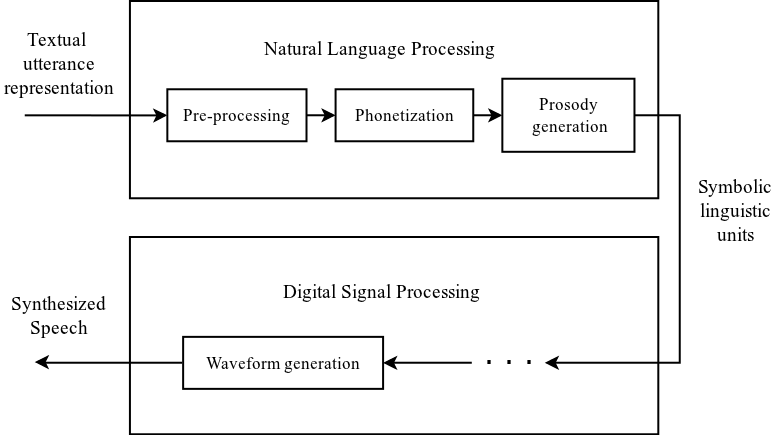
\includegraphics[width=0.9\columnwidth]{tts_con} 
    \caption{Componenti funzionali di un sintetizzatore}
\end{figure}

%**************************************************************

\section{Heterogeneous Relation Graph}
\subsection{Descrizione della struttura dati}
L'\textit{engine} di \textbf{Speect} rappresenta al suo interno l'\textit{utterance} tramite una struttura dati detta
\textbf{Heterogeneous Relation Graph} (HRG), ossia un grafo i cui nodi (detti \texttt{item}) sono organizzati per livelli
(detti \texttt{relation}). \\ Il sistema fornisce numerosi metodi per accedere al grafo e spostarsi all'interno dei suoi nodi,
anche attraverso le \textit{relation}. \\ Le \textit{relation} che costituiscono il grafo sono le seguenti:
\begin{itemize}
\item \texttt{Token}, è costituita da \textit{item} contenenti i \textit{token} dell'\textit{utterance};
\item \texttt{Word}: è costituita da \textit{item} contenenti le \textit{word} dell'\textit{utterance};
\item \texttt{Syllable}: è costituita da \textit{item} contenenti le sillabe che costituiscono le \textit{word};
\item \texttt{Segment}: è costituita da \textit{item} contenenti i fonemi delle \textit{word};
\item \texttt{SylStructure}: è una \textit{relation} che connette le tre \textit{relation} precedenti. \\
I nodi possono contenere anche informazioni aggiuntive chiamate \textit{feature}, calcolate dai \textit{feature processor}.
\end{itemize}

\subsection{Attraversamento del grafo}
Come si deduce dalla figura 3.2, le \textit{relation} \texttt{Word}, \texttt{Syllable} e \texttt{Segment} sono formate
da \textit{item} (tutti connessi) organizzati sotto forma di liste doppiamente concatenate attraversabili in entrambe le direzioni a partire da ogni nodo. \\
Dunque in queste tre \textit{relation} le uniche operazioni permesse per cambiare posizione rispetto ad un \textit{item} sono:
    \begin{enumerate}
      \item \texttt{next}: accesso all'\textit{item} successivo;
      \item \texttt{previous}: accesso all'\textit{item} precedente.
    \end{enumerate}
Diversamente dalle due \textit{relation} precedenti, la \textit{relation} \texttt{SylStructure}, come si vede dalla figura, 
non prevede che i suoi \textit{item} siano tutti connessi, ma fornisce altre due operazioni per la navigazione dei suoi nodi:
    \begin{enumerate}
      \item \texttt{daughter}: ogni \textit{item} può avere zero o più nodi figli;
      \item \texttt{parent}: ogni \textit{item} possiede uno e un solo nodo padre.
    \end{enumerate}

\subsection{Unicità degli item e condivisione del contenuto}
Gli \textit{item} sono univoci all'interno del grafo, tuttavia, nel caso in cui vi sia una sovrapposizione di contenuto tra 
due \textit{item} in due \textit{relation} distinte, questi sono considerati logicamente equivalenti. \\
In particolare, sempre facendo riferimento alla figura 3.2, si può notare come gli \textit{item} nella \textit{relation} \texttt{Word}
condividano il contenuto con gli \textit{item} al livello superiore della \textit{relation} \texttt{SylStructure}. Questa equivalenza
viene sfruttata per cambiare \textit{relation} durante l'attraversamento del grafo.

\begin{figure}[!h] 
    \centering 
    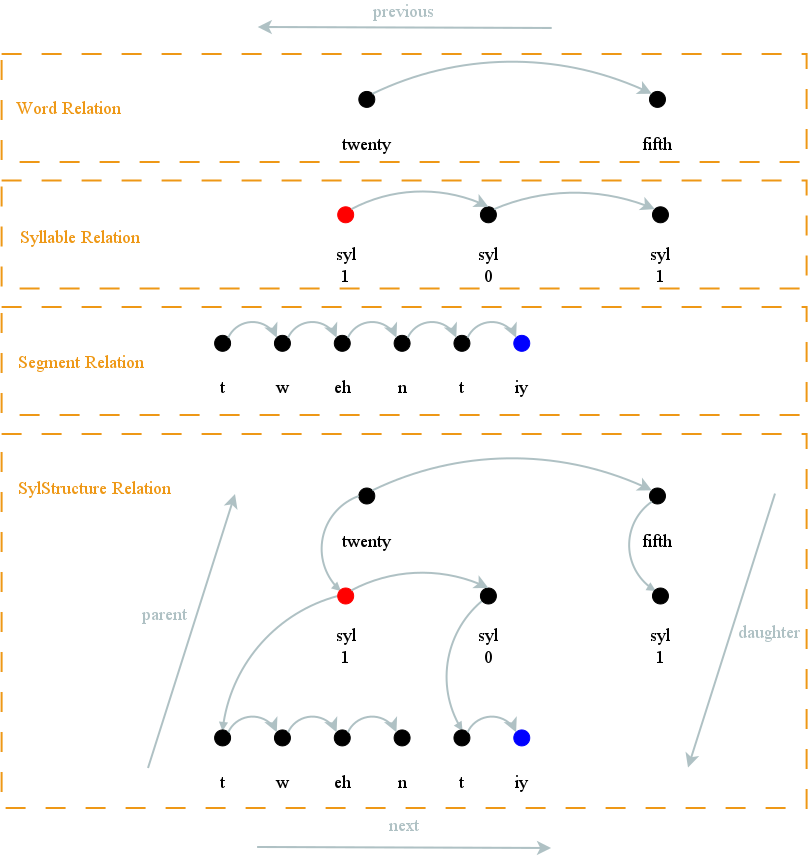
\includegraphics[width=0.9\columnwidth]{hrg} 
    \caption{Esempio di \textbf{H}eterogeneous \textbf{R}elation \textbf{G}raph}
\end{figure}



             % Kick-Off
%% !TEX encoding = UTF-8
% !TEX TS-program = pdflatex
% !TEX root = ../tesi.tex
% !TEX spellcheck = it-IT

%**************************************************************
\chapter{Analisi dei requisiti}
\label{cap:boh}
%**************************************************************

%\intro{}\\
\section{Forest useful snippet for  mivoq-nlp-scripts}

\begin{forest}
 for tree={
    font=\ttfamily,
    grow'=0,
    child anchor=west,
    parent anchor=south,
    anchor=west,
    calign=first,
    edge path={
      \noexpand\path [draw, \forestoption{edge}]
      (!u.south west) +(7.5pt,0) |- node[fill,inner sep=1.25pt] {} (.child anchor)\forestoption{edge label};
    },
    before typesetting nodes={
      if n=1
        {insert before={[,phantom]}}
        {}
    },
    fit=band,
    before computing xy={l=15pt},
  }
[mivoq-nlp-scripts
  [AUTHORS
    %[text1.1.1]
    %[text1.1.2]
    %[text1.1.3]
  ]
  [README.md
    %[text1.2.1]
    %[text1.2.2]
  ]
  [bin]
  [experiments]
  [lib]
  [test]
  [xsl]
]
\end{forest}

%Nelle tabelle \ref{tab:requisiti-funzionali}, \ref{tab:requisiti-qualitativi} e \ref{tab:requisiti-vincolo} sono riassunti i requisiti e il loro tracciamento con gli% use case delineati in fase di analisi.

\newpage
\section{Forest useful snippet for syllabification plugin}
\begin{forest}
  for tree={
    font=\ttfamily,
    grow'=0,
    child anchor=west,
    parent anchor=south,
    anchor=west,
    calign=first,
    edge path={
      \noexpand\path [draw, \forestoption{edge}]
      (!u.south west) +(7.5pt,0) |- node[fill,inner sep=1.25pt] {} (.child anchor)\forestoption{edge label};
    },
    before typesetting nodes={
      if n=1
        {insert before={[,phantom]}}
        {}
    },
    fit=band,
    before computing xy={l=15pt},
  }
[syllabification
  [AUTHORS
  %  [text1.1.1]
  %  [text1.1.2]
  %  [text1.1.3]
  ]
  [README
    %[text1.2.1]
    %[text1.2.2]
  ]
  [CMakeLists.txt]
  [Doxyfile]
  [cmake
     [sources.cmake]
  ]
  [src
     [ita\_it\_mivoq.h]
     [ita\_it\_mivoq.c]
     [plugin.c]
  ]
]
\end{forest}

\section{Forest useful snippet for rule based features plugin}
\begin{forest}
  for tree={
    font=\ttfamily,
    grow'=0,
    child anchor=west,
    parent anchor=south,
    anchor=west,
    calign=first,
    edge path={
      \noexpand\path [draw, \forestoption{edge}]
      (!u.south west) +(7.5pt,0) |- node[fill,inner sep=1.25pt] {} (.child anchor)\forestoption{edge label};
    },
    before typesetting nodes={
      if n=1
        {insert before={[,phantom]}}
        {}
    },
    fit=band,
    before computing xy={l=15pt},
  }
[rule\_based\_features]
  [AUTHORS
  %  [text1.1.1]
  %  [text1.1.2]
  %  [text1.1.3]
  ]
  [README
    %[text1.2.1]
    %[text1.2.2]
  ]
  [CMakeLists.txt]
  [Doxyfile]
  [cmake
     [sources.cmake]
  ]
  [src
     [rule\_based\_features.h]
     [rule\_based\_features.c]
     [plugin.c]
  ]
]
\end{forest}



%\begin{table}%
%\caption{Tabella del tracciamento dei requisti funzionali}
%\label{tab:requisiti-funzionali}
%\begin{tabularx}{\textwidth}{lXl}
%\hline\hline
%\textbf{Requisito} & \textbf{Descrizione} & \textbf{Use Case}\\
%\hline
%RFN-1     & L'interfaccia permette di configurare il tipo di sonde del test & UC1 \\
%\hline
%\end{tabularx}
%\end{table}%

%\begin{table}%
%\caption{Tabella del tracciamento dei requisiti qualitativi}
%\label{tab:requisiti-qualitativi}
%\begin{tabularx}{\textwidth}{lXl}
%\hline\hline
%\textbf{Requisito} & \textbf{Descrizione} & \textbf{Use Case}\\
%\hline
%RQD-1    & Le prestazioni del simulatore hardware deve garantire la giusta esecuzione dei test e non la generazione di falsi negativi & - \\
%\hline
%\end{tabularx}
%\end{table}%

%\begin{table}%
%\caption{Tabella del tracciamento dei requisiti di vincolo}
%\label{tab:requisiti-vincolo}
%\begin{tabularx}{\textwidth}{lXl}
%\hline\hline
%\textbf{Requisito} & \textbf{Descrizione} & \textbf{Use Case}\\
%\hline
%RVO-1    & La libreria per l'esecuzione dei test automatici deve essere riutilizzabile & - \\
%\hline
%\end{tabularx}
%\end{table}%
             % Concept Preview
% !TEX encoding = UTF-8
% !TEX TS-program = pdflatex
% !TEX root = ../tesi.tex
% !TEX spellcheck = it-IT

%**************************************************************
\chapter{Progettazione e realizzazione}
\label{cap:progettazione-realizzazione}
%**************************************************************

%\intro{}\\

%**************************************************************
%**************************************************************
%**************************************************************

\section{Strumenti utilizzati}
  \subsection{Hardware e sistema operativo}	  
    Il lavoro sul progetto non ha richiesto particolari risorse \textit{hardware}, ed ho potuto	
    utilizzare il mio portatile con Linux Ubuntu 14.04 (\textit{Trusty Tahr}) per lo sviluppo, nonostante questo
    non fosse un requisito obbligatorio per lavorare sul progetto; infatti \textbf{Speect} è un sistema portabile
    su tutte le maggiori piattaforme.
  \subsection{Linguaggi di programmazione e librerie esterne}
   L'\textit{engine} di \textbf{Speect} è sviluppato interamente in linguaggio \textit{C}, e permette di sviluppare i \textit{plug-in}
   in \textit{C} o in \textit{Python}. Durante questo \textit{stage} è stato utilizzato il linguaggio \textit{C}. \\
   Oltre al \textit{C} sono stati utilizzati i linguaggi \textit{bash} per l'attività di \textit{testing} e \hyperref[glo:xsl]{\emph{XSL}\glsfirstoccur}
   per l'elaborazione
   di alcuni \textit{file} \textit{XML} generati da alcuni processi di \textbf{Speect}. \\ 
   L'unica libreria esterna utilizzata nel progetto è \href{http://xmlsoft.org/}{LibXML2}, utilizzata nel \textit{plug-in} 
   \texttt{maryxml} per scrivere parte del contenuto dell' \textit{HRG} nel formato di \textit{output} definito 
   da \textbf{MaryTTS}, \href{http://mary.dfki.de/documentation/maryxml/}{MaryXML}. È stata scelta per i seguenti motivi:
   \begin{itemize}
      \item è scritta in \textit{C};
      \item è molto utilizzata;
      \item è rilasciata con \textit{licenza MIT}, la stessa con cui è rilasciato \textbf{Speect}.
   \end{itemize}

  \subsection{Strumenti per il \textit{building}} 
    \begin{itemize}
	\item \textbf{CMake}: è un generatore di sistemi di compilazione \textit{cross-platform}. Un progetto che utilizza questo \textit{tool} deve specificare
	      		      il processo di \textit{build} tramite dei \textit{file} indipendenti dalla piattaforma chiamati \texttt{CMakeLists.txt}, i quali 
			      devono far parte di ciascuna cartella dell'albero delle \textit{directory} del progetto;

        \item \textbf{Automake}: è un \textit{tool} per la generazione automatica di \textit{file} chiamati \texttt{Makefile.in} a partire
	      			 da \textit{file} chiamati \texttt{Makefile.am}. Questi contengono delle liste di definizioni di variabili
				 per il programma \textit{make} e di regole. I \textit{file} \texttt{Makefile.am} sono compatibili con gli 
				 \textit{standard} \textbf{GNU Makefile};
	\item \textbf{Autoconf}: è un \textit{tool} creato da \textit{GNU} che permette la creazione di pacchetti generando uno \textit{script bash}
                                 (chiamato \texttt{configure}) a partire da un \textit{file} chiamato \texttt{configure.ac},
	      			 il quale a sua volta è in grado di produrre un \textit{file} \texttt{Makefile}.
    \end{itemize}

   \subsection{Versionamento}
      \begin{figure}[!h] 
        \centering 
        
\includegraphics[width=0.5\columnwidth]{git-logo} 
        \caption{Logo di \textit{git}}
      \end{figure} 

      Per il controllo di versione l'azienda utilizza il \textit{software} \textit{git}, abbinato ai seguenti servizi per l'\textit{hosting}: 
      \begin{enumerate}
	\item \textbf{GitHub}: utilizzato per l'\textit{hosting} di un \textit{repository} pubblico contenente il codice 
	      		       di \textbf{Speect};
	\item \textbf{GitLab}: utilizzato per l'\textit{hosting} di un \textit{repository} privato contenente alcuni 
	      		       \textit{tool} interni all'azienda  per il \textit{building} ed il \textit{testing} di \textbf{Speect}.

	\paragraph{Workflow per git}
        Per quanto riguarda il \textit{workflow} nell'utilizzo di \textit{git} e \textit{GitHub}, la politica aziendale impone
	di creare un \textit{fork} del \textit{repository} dell'azienda e di contribuire al progetto da tale \textit{fork}.
	Pertanto ho sempre eseguito i \textit{commit} ed i \textit{push} avendo come riferimento il mio \textit{fork} personale;
	il codice da me prodotto è stato sempre integrato dal \textit{tutor} aziendale nel \textit{repository} dell'azienda tramite
 	\textit{rebasing}. \\ Le norme da seguire nella partecipazione al progetto sono state dunque le seguenti:
        \begin{itemize}
           \item un \textit{commit} deve riguardare un singolo \textit{file}, e le modifiche contenute in esso
              devono avere un unico obiettivo;
           \item una volta terminato un \textit{task}, si effettua un \textit{push} sul \textit{fork} personale;
           \item si effettua una richiesta di integrazione all'integratore (nel nostro caso al \textit{tutor} aziendale), il quale
                 può:
                    \begin{itemize}
                      \item accettarla ed integrare i \textit{commit} nel \textit{fork} principale del progetto;
                      \item rifiutarla e richiedere modifiche ai \textit{commit}.
                    \end{itemize}
        \end{itemize}
        
      \end{enumerate}

%*************************************

\section{Il \textit{plug-in} maryxml}
Come introduzione al sistema e ai \textit{plug-in} mi è stato chiesto di effettuare alcune modifiche
al \textit{plug-in} \texttt{maryxml}, il quale è stato creato dai due tirocinanti precedenti con lo scopo
di confrontare l'\textit{output} generato da \textbf{Speect} con l'\textit{output} di \textbf{MaryTTS}.
   \subsection{Il formato \textit{MaryXML}}
      \textbf{MaryTTS} utilizza il metalinguaggio \textit{XML} per la trattazione dei dai interni. \\
             Il linguaggio definito tramite \textit{XML Schema} all'interno di \textbf{MaryTTS} prende il nome
             di \textit{MaryXML}. L'utilizzo di \textit{XML} comporta i seguenti:
                  \begin{itemize}
                    \item vantaggi:
                         \begin{itemize}
                            \item rigidità fornita dal metalinguaggio;
                            \item facilità nel manipolare i dati;
                            \item possibilità di avere \textit{file} sempre validi.
                         \end{itemize}
                    \item svantaggi:
                         \begin{itemize}
                           \item impossibilità da parte degli utenti di modificare gli schemi;
                           \item le modifiche sono possibili soltanto negli schemi locali.
                         \end{itemize}
                  \end{itemize}
                  \textbf{MaryTTS} utilizza il linguaggio \textit{MaryXML} per tutti i \textit{file} interni,
                  compresi quelli riguardanti la voce. In \textbf{MaryTTS}, ogni lista di fonemi, dizionario o rappresentazione
                  dei \textit{token} deve seguire lo schema definito per \textit{MaryXML}. \\ Data la rigidità dello schema, l'aggiunta
                  di nuovi elementi o attributi è possibile solamente dopo le modifiche degli \textit{schema} locali 
                  e delle classi per la lettura dei nuovi elementi/attributi. \\
                  In \hyperref[app:appc]{Appendice C} viene riportato un esempio di \textit{file} \textit{MaryXML}.
                  \paragraph{Nota su Speect} A differenza di \textbf{MaryTTS}, \textbf{Speect} per trattare
                  i \textit{file} interni utilizza il linguaggio \textit{JSON}, il quale permette di fornire
                  maggiore libertà all'utente definendo un numero ristretto di regole.
         \subsection{Scopo del \textit{plug-in}}
             Il \textit{plug-in} ha lo scopo di scrivere su \textit{file} i \textit{token} generati e normalizzati
             di \textbf{Speect}. \\
             Sostanzialmente questa componente richiede all'\textit{HRG} i \textit{token} da stampare e li scrive su \textit{file} 
             in formato \textit{MaryXML}. \\
             Prima del mio \textit{stage} non venivano stampati i dati riguardanti le sillabe, dunque il mio contributo
             a questo \textit{plug-in} consiste nell'aver ricavato questi dati dall'\textit{HRG} e nell'averli stampati
             in formato \textit{MaryXML}. \\
             Di seguito vengono riportati due \textit{output} provenienti dall'elaborazione dell'\textit{input} 'Ciao' 
             (rispettivamente prima e dopo il mio contributo):
             \begin{itemize}
               \item \textit{senza} i dati relativi alle sillabe: \\
                 \begin{lstlisting}[language=XML] 
                   <t pos="SP" ph="tS a - o">ciao</t> 
                 \end{lstlisting}
               \item \textit{con} i dati relativi alle sillabe: \\
                 \begin{lstlisting}[language=XML] 
                   <t pos="SP" ph="tS a - o">ciao<syllable><ph p="tS"/><ph p="a"/></syllable><syllable><ph p="o"/></syllable></t>
                 \end{lstlisting}
             \end{itemize}
%*************************************

\section{Sviluppo del sillabificatore}
\label{sec:progettazione}
All'inizio del periodo di \textit{stage} \textbf{Speect} non includeva tra i suoi \textit{utterance processor} un sillabificatore
per la lingua italiana, perciò negli esperimenti dell'azienda gli \textit{input} in lingua italiana venivano sillabificati secondo le regole
della lingua inglese, riducendo così la qualità dell'\textit{output} prodotto.
%Marina Nespor, "Le strutture del linguaggio - Fonologia"
%Pietro Maturi, "I suoni delle lingue, i suoni dell'italiano"
%T.A. Hall, "English syllabification as the interaction of markedness constraints", Studia Linguistica, vol. 60, 2006, pp. 1-33 --> link
%https://www.researchgate.net/publication/227729497_English_syllabification_as_the_interaction_of_markedness_constraints
\subsection{I due approcci alla sillabificazione}
Tradizionalmente il problema della sillabificazione è affrontato definendo delle sequenze di fonemi (dette \textit{cluster}) valide per 
una determinata lingua, e definendo regole di sillabificazione opportune sulla loro base. \\ Per l'implementazione del sillabificatore
il \textit{tutor} aziendale ha proposto un algoritmo basato sulla variazione della sonorità dei fonemi che riduce la necessità di 
codificare esplicitamente i \textit{cluster} di fonemi di una lingua.
      \subsubsection{Sillabificazione per \textit{cluster}}
           È il metodo utilizzato dal \textit{plug-in} già esistente in \textbf{Speect} per l'inglese, teorizzato
           nell'articolo 
           \href{http://www.zas.gwz-berlin.de/fileadmin/material/ZASPiL_Volltexte/zp37/zaspil37-hall.pdf}
           {\textit{English syllabification as the interaction of markedness constraints}} di T.A. Hall. \\
           Quest'ultimo propone delle azioni predefinite in base ai \textit{cluster} di fonemi incontrati nella stringa di \textit{input} durante il suo \textit{parsing}. \\
           Nella trattazione seguente verranno utilizzati i seguenti simboli:
           \begin{itemize}
             \item \textbf{C}: rappresenta una consonante;
             \item \textbf{G}: rappresenta una semivocale;
             \item \textbf{V}: rappresenta un picco di sonorità all'interno di una sillaba, che può consistere in:
                               \begin{itemize}
                                 \item una \textit{vocale breve};
                                 \item una \textit{vocale lunga};
                                 \item un \textit{dittongo};
                                 \item una \textit{sonorante sillabica}.
                               \end{itemize}
           \end{itemize}
           Nella seguente tabella vengono riportati alcuni esempi di regole tratti dall'articolo citato (il simbolo '.' viene usato come
           separatore tra le sillabe): \newpage
           %BEGIN of table section
           \begin{center}
             \begin{longtable}{ | >{\centering}p{2cm} | >{\centering}p{4cm} | >{\centering}p{1.5cm} | >{\centering}p{2cm} | }
               \hline
               \textbf{Cluster} & \textbf{Possibili sillabificazioni} \tabularnewline \hline
                % example & bla \tabularnewline \hline
                 VCV & V\textbf{.}CV  \tabularnewline \hline
                 VCCV & V\textbf{.}CCV, VC\textbf{.}CV  \tabularnewline \hline
                 VCCCV & VC\textbf{.}CCV, VCC\textbf{.}CV  \tabularnewline \hline
                 VCCCCV & VC\textbf{.}CCCV  \tabularnewline \hline
                 VCGV & VC\textbf{.}GV, V\textbf{.}CGV, VC\textbf{.}GV  \tabularnewline \hline
                 VCCGV & V\textbf{.}CCGV  \tabularnewline \hline
                 VCCCGV & VC\textbf{.}CCGV  \tabularnewline \hline
             \end{longtable}
           \end{center}
           %END of table section
         %  \begin{itemize} 
             \paragraph{Vantaggi} 
               Il presente metodo è abbastanza semplice da implementare, inoltre è ben documentato nell'articolo di T.A. Hall.
             \paragraph{Svantaggi} 
               Gli svantaggi principali della sillabificazione per \textit{cluster} sono la verbosità nella sua implementazione
               e il comportamento non definito in caso di \textit{input} non ben formati secondo le regole della lingua in esame.  
         %  \end{itemize}
      \\
      \subsubsection{Sillabificazione per sonorità} 
      Il metodo si basa su alcuni semplici principi riguardanti la sonorità dei fonemi all'interno di una sillaba, proposti da 
      Pietro Maturi in \href{https://www.mulino.it/isbn/9788815133052}{\textit{I suoni delle lingue, i suoni dell'italiano}}. \\
      Di questo algoritmo esistono due sole implementazioni, una parziale in \textit{Java} di Giulio Paci (il \textit{tutor} aziendale), 
      e quella discussa in questo documento, completa e in \textit{C}.
      Innanzitutto viene stabilita una \textit{scala di sonorità} dei fonemi in base alla loro tipologia, presentata qui in ordine
      di sonorità crescente dal primo all'ultimo elemento della lista:
      \begin{enumerate}
        \item {\hyperref[glo:consoccl]{consonanti \emph{occlusive}\glsfirstoccur}};
        \item {\hyperref[glo:consfric]{consonanti \emph{fricative}\glsfirstoccur}};
        \item {\hyperref[glo:consnasa]{consonanti \emph{nasali}\glsfirstoccur}};
        \item {\hyperref[glo:conslate]{consonanti \emph{laterali}\glsfirstoccur}};
        \item \textit{s sorda}: questo fonema viene trattato singolarmente in questa posizione per evitare
          l'introduzione di ulteriori regole proposte nell'articolo di Maturi.\\  Di fatto questo trattamento per
          la 's sorda' elimina anche la necessità di utilizzare alcuni \textit{cluster} proposti nello stesso articolo;
        \item {\hyperref[glo:consvibr]{consonanti \emph{vibranti}\glsfirstoccur}};
        \item {\hyperref[glo:consappr]{consonanti \emph{approssimanti}\glsfirstoccur}};
        \item vocali.
      \end{enumerate}
      Una parola è dunque costituita dall'alternanza di suoni più o meno \textit{intensi},
      per cui l'algoritmo di sillabificazione per sonorità può
      essere riassunto nel modo seguente: \\ \\
         %   \begin{center}
                \texttt{Data una lista di zero o più consonanti comprese tra due vocali v1 e v2, il punto di inizio della sillaba
                   contenente v2 è situato nel punto in cui la sonorità non decresce spostandosi nel verso che va da v2
                   a v1.} \\ \\
        %    \end{center}
          
      %La seguente immagine dovrebbe rendere più chiaro il funzionamento di questo metodo: 
      % serve un'immagine di una parola con le frecce
      % \begin{figure}[!h] 
      %  \centering 
      %  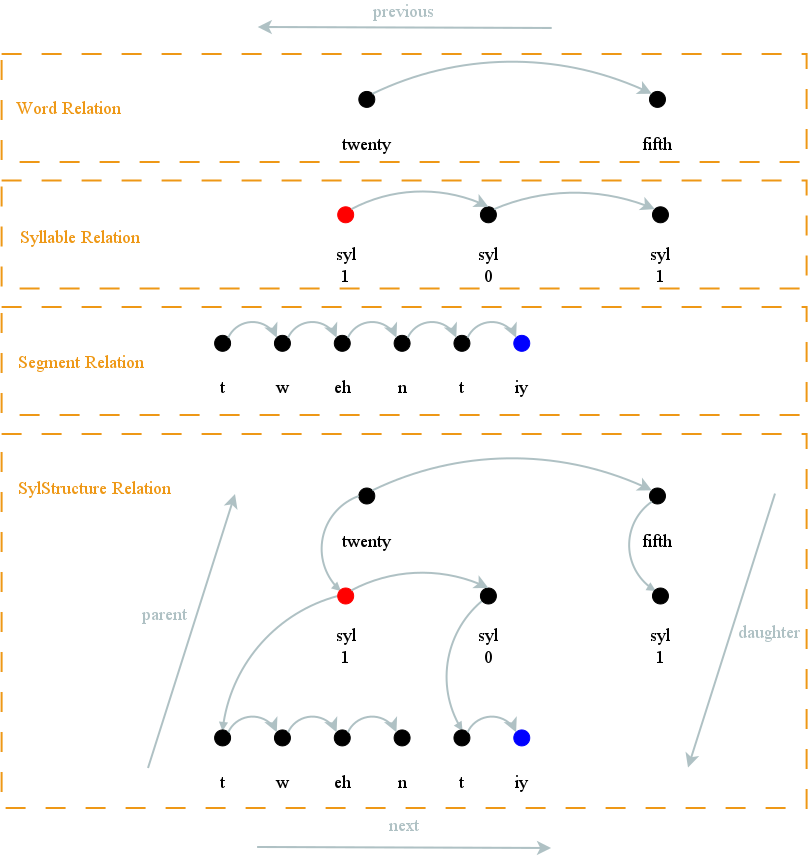
\includegraphics[width=0.9\columnwidth]{hrg} 
      %  \caption{Esempio di \textbf{H}eterogeneous \textbf{R}elation \textbf{G}raph}
      %  \end{figure}
      Questo metodo funziona nella maggior parte dei casi, tuttavia l'attività di \textit{testing} ha permesso 
      di individuare dei casi (gestiti con opportune eccezioni)
      in cui l'algoritmo fornito sopra produce \textit{output} scorretti:
      \begin{itemize}
        \item {\hyperref[glo:consappr]{consonanti \emph{approssimanti}\glsfirstoccur}} adiacenti: 
              i due fonemi devono rientrare nella stessa sillaba;
              \label{exc:apprappr}
        \item {\hyperref[glo:consoccl]{consonante \emph{occlusiva}\glsfirstoccur}} seguita da una 
              {\hyperref[glo:consnasa]{consonante \emph{nasale}\glsfirstoccur}}: i due fonemi devono appartenere a due sillabe diverse;
              \label{exc:occlnasa}
        \item {\hyperref[glo:consoccl]{consonante \emph{occlusiva}\glsfirstoccur}} seguita da un'altra 
              {\hyperref[glo:consoccl]{consonante \emph{occlusiva}\glsfirstoccur}}: i due fonemi devono appartenere a due sillabe diverse;
              \label{exc:occloccl}
        \item {\hyperref[glo:conslate]{consonante \emph{laterale}\glsfirstoccur}} seguita dalla consonante \textit{s}: 
              i due fonemi devono appartenere a due sillabe diverse;
              \label{exc:lates}
        \item {\hyperref[glo:consnasa]{consonante \emph{nasale}\glsfirstoccur}} seguita dalla consonante \textit{s}: 
              i due fonemi devono appartenere a due sillabe diverse.
              \label{exc:nasas} 
      \end{itemize}

           %\begin{itemize}
             \paragraph{Vantaggi}
                     È molto meno verboso rispetto al metodo precedente, fatto che si concretizza in una dimensione del codice molto
                     più ridotta (la riduzione del numero di righe di codice è stata del 65\%). \\ Inoltre permette di gestire 
                     qualsiasi \textit{input}, compresi
                     quelli che non rispettano le regole della lingua in esame.
             \paragraph{Svantaggi}
                    L'implementazione di questo algoritmo richiede maggiore attenzione rispetto alla sillabificazione per \textit{cluster}.
           %\end{itemize}



%**************************************************************

%**************************************************************
\section{Calcolo e raccolta delle \textit{feature}}
I \textit{feature processor} hanno lo scopo di calcolare alcuni attributi propri di varie componenti dell'\textit{input},
tra cui fonemi, sillabe e frasi, attributi che in seguito verranno scritti come campi dati degli \textit{item} del grafo \textit{HRG}. \\
Esempi di \textit{feature} sono i seguenti (di seguito ne vengono riportate soltanto le descrizioni testuali):
\begin{itemize}
  \item livello \textit{phrase}: numero di \textit{phrase} successive a quella corrente nell'\textit{utterance};
  \item livello \textit{phoneme}: {numero di \textit{phoneme} successivi a quello corrente dentro la sillaba}.
\end{itemize}

Le \textit{feature} calcolate dai \textit{feature processor} sono utili in quanto vengono sfruttate dal \textit{vocoder} per
la sintesi dell'\textit{input} fornitogli dal \textit{front-end}. Il \textit{vocoder} di cui fa uso attualmente \textbf{Speect} è 
\href{http://hts-engine.sourceforge.net/}{HTS engine}. \\ 
Tuttavia \href{http://hts-engine.sourceforge.net/}{HTS engine} richiede che le \textit{feature} gli siano passate sotto forma di codici 
alfanumerici, da qui in poi denominati \textit{htslabel}. In generale le \textit{htslabel} sono delle etichette arbitrarie, ma, poiché vengono
utilizzate dal \textit{back-end} come chiavi di ricerca all'interno di un \textit{database} per trovare i parametri necessari alla produzione di audio, 
esse devono avere lo stesso formato di quelle utilizzate durante la fase di creazione dei \textit{database}. Per poter utilizzare i \textit{database} 
di cui si serve \textbf{MaryTTS} è perciò necessario effettuare una mappatura tra i nomi 
delle \textit{feature} in \textbf{Speect} e i codici \textit{hts} corrispondenti definiti da \textbf{MaryTTS} (parte dell’attività di mappatura era 
già stata svolta prima dello \textit{stage}). \\
Sono stati dunque corretti ed ampliati due \textit{plug-in}, \texttt{hts\_label\_data\_collector} e \texttt{hts\_label\_generator\_it}.

\begin{figure}[!h] 
    		\centering 
    		
\includegraphics[width=0.4\columnwidth]{hts_logo} 
   	 	\caption{Logo di \textit{HTS engine}}
\end{figure}


      \subsection{Il \textit{plug-in} hts\_label\_data\_collector}
		Il \textit{plug-in} era già in uno stadio avanzato (se si esclude un \textit{segmentation fault} causato
                da un'istruzione di \textit{return} mancante) prima dello \textit{stage}. \\
		Sostanzialmente esso costituisce un \textit{hub} avente il compito di ricavare i dati dai 
                \textit{feature processor} disponibili
		e di scrivere i nomi e i valori delle \textit{feature} da essi calcolate nei nodi dell'\textit{HRG}. \\
                I nomi delle \textit{feature} sono del tutto arbitrari (infatti sono stati stabiliti da un altro tirocinante),
		ma univoci, in quanto devono poter essere usati come chiavi per la ricerca dei valori corrispondenti. \\
                La tabella 4.2 riporta le relazioni tra alcune \textit{feature} e alcuni \textit{feature processor}, con le descrizioni
                del significato delle \textit{feature}.
                \newpage
                %COMMENTO: serve una tabella con qualche feature e il plugin usato per calcolarla,
		%COMMENTO: negli appunti 20_06.txt ci sono le associazioni
		\begin{center}
        		\bgroup
        		\def\arraystretch{1.8}
        		\begin{longtable}{ | l | p{2cm} | p{4.7cm} | p{2.5cm} |}
        		\hline
        		\textbf{Feature} & \textbf{Descrizione}
        		& \textbf{Feature Processor} \\ \hline
        		\texttt{phrase.syls.num} & numero di sillabe nella \textit{phrase} & \texttt{phrase\_num\_syls} \newline  \\ \hline
        		\texttt{phrase.words.num} & numero di \textit{word} nella \textit{phrase} & \texttt{phrase\_num\_words} \newline  \\ \hline
       			\texttt{phrases.from.utt.end} & numero di \textit{phrase} successive a quella corrente nell'\textit{utterance}  & \texttt{phrase\_pos\_utt\_rev} \newline  \\ \hline
        		\texttt{phrases.from.utt.start} & numero di \textit{phrase} successive a quella corrente nell'\textit{utterance} & \texttt{phrase\_pos\_utt} \newline  \\ \hline
         
        		\texttt{phones.from.syl.end} & numero di \textit{phoneme} successivi a quello corrente dentro la sillaba & \texttt{segment\_pos\_syl\_end} \newline  \\ \hline
        		\texttt{phones.from.syl.start} & numero di \textit{phoneme} precedenti a quello corrente dentro la sillaba & \texttt{segment\_pos\_syl} \newline  \\ \hline
       			\texttt{utterance.phrases.num} & numero di \textit{phrase} nella \textit{utterance} corrente & \texttt{utt\_num\_phrases}  \newline  \\ \hline
        	 	\texttt{syl.phones.num} & numero di \textit{phoneme} nella sillaba corrente & \texttt{syllable\_num\_phones} \newline  \\ \hline                 

       			\texttt{syls.from.phrase.end} & numero di sillabe nella \textit{phrase} corrente & \texttt{syllable\_pos\_phrase\_rev}  \newline  \\ \hline
        		\texttt{syls.from.phrase.start} & numero di sillabe precedenti a quella corrente nella \textit{phrase}  & \texttt{syllable\_pos\_phrase} \newline  \\ \hline
       			\texttt{syls.from.prev.accent} & numero di sillabe successive all'ultima sillaba accentata & \texttt{syllable\_accent\_all\_in} \newline  \\ \hline

        	        \caption{Feature e Feature Processor}
        	        \end{longtable}
        	        \egroup
     	        \end{center}
    	%END of table
     \subsection{Il \textit{plug-in} hts\_label\_generator\_it}
		 Questo \textit{plug-in} si occupa della costruzione dell'\textit{output} per \textit{HTS engine} ricavando i dati
		 necessari  dal \textit{plug-in} precedente. \\ Sostanzialmente esso si occupa di invocare il \textit{plug-in}
		 \texttt{hts\_label\_data\_collector} e di salvare i dati da esso raccolti in una stringa, la quale 
		 in seguito verrà mandata in \textit{output} su \textit{file}.  \\
		 La struttura e le funzionalità di base del presente \textit{plug-in} erano già state sviluppate
		 da un altro tirocinante, tuttavia sono state apportate le seguenti modifiche:
		 \begin{itemize}		
			\item molte \textit{feature} calcolate dal \textit{plug-in} \texttt{hts\_label\_data\_collector}
			      non venivano effettivamente utilizzate e quindi non risultavano nell'\textit{output}
			      finale: si è dunque provveduto a ricavare una parte significativa delle \textit{feature}
			      calcolate. \\ Lo scopo primario di tale attività è stato generare un \textit{output}
			      con il maggior numero possibile di informazioni, fornendo così a \textit{HTS engine} un \textit{input}
			      più completo;
			\item analizzando il codice esistente del presente \textit{plug-in} è stato notato come i nomi
			      delle \textit{feature} (all'interno di \textbf{Speect}) e i codici \textit{hts} corrispondenti
			      fossero presenti come stringhe all'interno del codice. \\ È stato dunque considerato opportuno
			      un certo grado di parametrizzazione, ponendo la mappatura tra nomi in \textbf{Speect} e codici
			      \textit{hts} all'interno del \textit{file} di configurazione \texttt{voice.json}.
		 \end{itemize} 
                 La parametrizzazione del \textit{plug-in} citata sopra ha permesso di spostare il problema dell'aggiunta delle
                 \textit{feature} nella configurazione. \\ Questo fatto assume una grande importanza in quanto ora il \textit{plug-in} 
                 è generico: ciò significa che, a meno di correzioni e di piccoli miglioramenti, non è più necessario modificarlo
                 per estenderne l'\textit{output}; in questo modo l'estensione a nuove lingue e voci diventa più agevole
                 (in precedenza era necessario riscrivere il \textit{plug-in} per ogni impostazione). \\
                 Dunque, grazie a questa nuova impostazione, l'aggiunta di nuove \textit{feature} (se ricavate dal
                 \textit{plug-in} \texttt{hts\_label\_data\_collector})
                 non richiede più alcuna modifica del codice del presente \textit{plug-in}.


      \subsection{Utterance processor 'Prosody'}
                Per replicare le componenti di \textbf{MaryTTS} che calcolano le informazioni di intonazione prosodica è stato necessario 
                introdurre un nuovo \textit{plug-in}, \texttt{rule\_based\_features}, che implementasse un nuovo \textit{utterance processor} 
                chiamato \texttt{Prosody}. \\ Prima del mio \textit{stage} nessuna \textit{feature} era stata calcolata tramite questo metodo
                (per motivi di tempo i due tirocinanti precedenti e il \textit{tutor} aziendale non si sono dedicati a questo lavoro),
                pertanto la realizzazione del presente \textit{plug-in} ha previsto lo studio delle analoghe componenti di \textbf{MaryTTS},
                la progettazione della componente e la sua implementazione. \\
                
                \paragraph{Descrizione del metodo utilizzato}
                Il valore di alcune \textit{feature} può essere ricavato attraverso l'applicazione di semplici \textit{regole},
                le quali sono esprimibili nella seguente forma:
	\\ \\
          \texttt{Dato un nodo del grafo HRG, se esso è caratterizzato da una feature \textit{x} con valore \textit{v}, e questo
		  valore appartiene ad una lista \textit{Lv}, allora si può impostare una feature \textit{y} ad un valore \textit{w}. \\
		  Se la regola precedente fallisce, ne vengono applicate altre a cascata fino ad una regola che ha successo oppure fino
		  all'esaurimento di tutta la sequenza di regole.} \\ 

                L'\textit{engine} \textbf{MaryTTS} calcola alcune \textit{feature} tramite questo metodo,
                ma pone liste di valori e regole insieme all'interno
                di un \textit{file} di configurazione \textit{XML}. \\ Per l'implementazione di questo \textit{plug-in} è stato ritenuto opportuno	
                (almeno in una prima fase) mantenere separati i dati e le azioni corrispondenti alle regole. \\ Pertanto alcune liste di valori
                del \textit{file} \textit{XML} di \textbf{MaryTTS} citato sopra sono state riportate nel \texttt{voice.json}, tra i dati  
                associati all'\textit{utterance processor} \texttt{Prosody}.
                \paragraph{Esempi di regole}
                  \begin{itemize}
                    \item \textbf{regola sulla lista pos\_tonal\_accent}: se il valore della \textit{feature} 
                                                                          \texttt{POS} (che rappresenta il \texttt{part-of-speech tag} 
                                                                          associato all'\textit{item}) del \textit{word item} 
                                                                          è contenuto nella lista chiamata \texttt{pos\_tonal\_accent}
                                                                          (è una lista di valori contenuta nel \textit{file} di configurazione),
                                                                          allora il valore della \textit{feature} \texttt{accent} del \textit{word item}
                                                                          va impostato alla stringa \texttt{tone};
                    \item \textbf{regola sulla lista pos\_no\_accent}:    se il valore della \textit{feature} 
                                                                          \texttt{POS} (che rappresenta il \texttt{part-of-speech tag} 
                                                                          associato all'\textit{item}) del \textit{word item} 
                                                                          è contenuto nella lista chiamata \texttt{pos\_no\_accent}
                                                                          (è una lista di valori contenuta nel \textit{file} di configurazione),
                                                                          allora il valore della \textit{feature} \texttt{accent} del \textit{word item}
                                                                          va impostato alla stringa vuota;
                    \item \textbf{regola di default}:                     in caso di fallimento delle due regole precedenti,
                                                                          allora il valore della \textit{feature} \texttt{accent} del \textit{word item}
                                                                          va impostato alla stringa vuota;
                    \item \textbf{regole sul tipo di frase}:
                                         \begin{itemize}
                                           \item se il \textit{word item} fa parte di una \textit{phrase} con \textit{feature} 
                                             \texttt{type} impostata alla stringa \texttt{decl}, è associato
                                             ad una \texttt{prosodicPosition} con \texttt{type} impostato a \texttt{prenuclear},
                                             e la \textit{feature} \texttt{accent}
                                             è impostata alla stringa \texttt{tone} (ossia la stringa stabilita da una delle regole precedenti),
                                             allora il valore \texttt{tone} va sostituito con la stringa \texttt{L+H*};
                                           \item se la regola precedente fallisce ma valgono tutte le sue condizioni eccetto il fatto
                                                 che il \textit{word item} è associato
                                                 ad una \texttt{prosodicPosition} con \texttt{type} impostato a \texttt{nuclearNonParagraphFinal},
                                                 allora il valore \texttt{tone} va sostituito con la stringa \texttt{!H*}.
                                         \end{itemize}
                  \end{itemize}
             % Product Prototype
% !TEX encoding = UTF-8
% !TEX TS-program = pdflatex
% !TEX root = ../tesi.tex
% !TEX spellcheck = it-IT

%**************************************************************
\chapter{Verifica e validazione}
\label{cap:verifica-validazione}
%**************************************************************
%input example for syll_test: k o n t a m i n a1 n d o LL i s i
%output example for syll_text: k o n - t a - m i - n a1 n - d o - LL i - s i
\section{Testing del sillabificatore}
Il \textit{plug-in} di sillabificazione per l'italiano è stato associato fin dall'inizio della sua
progettazione ad un programma di verifica scritto sempre in \textit{C}. \\
 \subsection{Funzionamento del programma di test}
  Questo programma (che per comodità chiameremo \texttt{syll\_test}) riceve in \textit{input} su \texttt{stdin}
  (\textbf{st}andard \textbf{in}put) una sequenza di \textit{phoneme} rappresentante una parola per 
  ciascuna riga (prima colonna della tabella 5.1). \\
  Successivamente, dopo la lettura 
  da \texttt{stdin}  di una singola riga, si occupa di invocare il \textit{plug-in} di sillabificazione prestabilito
  all'interno del \textit{file} \texttt{voice.json}. \\ Infine, la lista di sillabe generata dal sillabificatore
  viene stampata su \texttt{stdout} (\textbf{st}andard \textbf{out}put), utilizzando il carattere '\textbf{-}' come separatore per le sillabe 
  (seconda colonna della   tabella 5.1). \\
  Il \textit{test} \texttt{syll\_test} è stato realizzato prima del sillabificatore, pertanto inizialmente l'\textit{input}
  è stato sillabificato utilizzando il sillabificatore per la lingua inglese. In questo modo è stato possibile accertare
  che lo stesso \textit{test} fosse corretto e conforme alle aspettative. \\
  Il \textit{tutor} aziendale mi ha fornito fin da subito due \textit{file}, rispettivamente di \textit{input} e 
  di \textit{output}, contenenti circa mille esempi di sequenze di fonemi e delle sillabificazioni attese.  \\ 
  Nella seguente tabella è possibile vedere alcuni esempi di \textit{input} (colonna di sinistra) e di
  \textit{output} (colonna di destra).
\begin{center}
        \bgroup
        \def\arraystretch{1.8}
        \begin{longtable}{ | l | p{2cm} | p{4.7cm} | p{2.5cm} |}
        \hline
        \textbf{Esempio input} & \textbf{Esempio output atteso} \\ \hline
        k a r o t a1 v a & k a - r o - t a1 - v a  \newline  \\ \hline
        a rr o t O1 & a - rr o - t O1 \newline  \\ \hline
        r i a1 nn o & r i - a1 - nn o \newline  \\ \hline
        r a1 d i k a & r a1 - d i - k a     \newline  \\ \hline
        s p O1 r t e & s p O1 r - t e   \newline  \\ \hline
        r i p a r t i1 t e &  r i - p a r - t i1 - t e   \newline  \\ \hline
        i n i m i k a1 t i & i - n i - m i - k a1 - t i   \newline  \\ \hline
        g r E1 v i & g r E1 - v i     \newline  \\ \hline
        \caption{Alcuni \textit{input} e \textit{output} attesi}
        \end{longtable}
        \egroup
     \end{center}
    %END of table
   \paragraph{Eccezioni nell'algoritmo di sillabificazione rilevate grazie a syll\_test}
       Nella seguente tabella vengono riportati alcuni risultati ricavati da \texttt{syll\_test}
       utili per una corretta implementazione dell'algoritmo di sillabificazione implementato 
       durante lo \textit{stage}. \\
       Le differenze tra le colonne 'Output' e 'Output atteso' hanno permesso di formulare
       le eccezioni dell'algoritmo di \textit{sillabificazione per sonorità} riportate nel
       {\hyperref[sec:progettazione]{quinto capitolo}}.
       %BEGIN of table
       %Tabella 
      \begin{center}
        \bgroup
        \def\arraystretch{1.8}
        \begin{longtable}{ | l | p{2cm} | p{4.7cm} | p{2.5cm} |}
        \hline
        \textbf{Input} & \textbf{Output senza eccezioni}
        & \textbf{Output atteso} \\ \hline
        %consonante nasale seguita dalla consonante s
        {\hyperref[exc:nasas]{i n s i s t i1 t a}} & i - n s i -  s t i1 - t a & i n - s i s - t i1 - t a \newline  \\ \hline
        %consonante laterale seguita dalla consonante s:
        {\hyperref[exc:lates]{r i v u l s i1 v a}} & r i - v u - l s i1 - v a & r i - v u l - s i1 - v a \newline  \\ \hline
        %consonante occlusiva seguita da un’altra consonante occlusiva
        {\hyperref[exc:occloccl]{a b d o1 tt i l i}} & a - b d o1 - tt i - l i & a b - d o1 - tt i - l i \newline  \\ \hline
        %consonante occlusiva seguita da una consonante nasale
        {\hyperref[exc:occlnasa]{s t i g m a t i1 ddz a}} & s t i - g m a - t i1 - ddz a & s t i g - m a - t i1 - ddz a \newline  \\ \hline
        %consonanti approssimanti [g] adiacenti 
        {\hyperref[exc:apprappr]{t r e ttS a j w O1 l o}} & t r e - ttS a j - w O1 - l o & t r e - ttS a - j w O1 - l o \newline  \\ \hline
        \caption{Eccezioni per l'algoritmo di sillabificazione}
        \end{longtable}
        \egroup
     \end{center}
    %END of table

       













\section{Test di unità}
Durante lo sviluppo sono stati realizzati alcuni \textit{test} di unità, scritti
in linguaggio \textit{bash}. \\
Gli \textit{script} di \textit{test} sono sempre composti da almeno tre \textit{test}:
  \begin{enumerate}
    \item un \textit{test} che termina \textbf{correttamente};
    \item un \textit{test} che \textbf{fallisce};
    \item un \textit{test} con \textit{output} \textbf{errato}.
  \end{enumerate}
A causa della loro importanza, alcuni \textit{test} sono stati scritti anche dal \textit{tutor} 
aziendale e da altri elementi dell'azienda. \\
La configurazione del \textit{file} \texttt{Makefile.am} permette di stabilire quali \textit{test} devono essere
eseguiti. \\ Dopo l'esecuzione di \textit{automake} è possibile lanciare le batterie di test tramite il
comando \texttt{make check}. \\
Ogni \textit{test} è preceduto e seguito da due funzioni:
\begin{itemize}
  \item \texttt{test\_start}: viene invocata prima di ogni \textit{test} di unità
                              con lo scopo di inizializzare le variabili utilizzate
                              in seguito nel \textit{test};
  \item \texttt{test\_end}:   controlla i risultati del \textit{test} e ripulisce l'ambiente
                              di \textit{testing}.
\end{itemize}
             % Product Design Freeze e SOP
% !TEX encoding = UTF-8
% !TEX TS-program = pdflatex
% !TEX root = ../tesi.tex
% !TEX spellcheck = it-IT

%**************************************************************
\chapter{Conclusioni}
\label{cap:conclusioni}
%**************************************************************

%**************************************************************
%\section{Consuntivo finale}

%**************************************************************
\section{Raggiungimento degli obiettivi}
A conclusione dello \textit{stage}, il \textit{front-end} per l'italiano per \textbf{Speect}
è stato sensibilmente migliorato, fornendo al \textit{back-end} un maggior numero di informazioni corrette,
confermando così che \textbf{Speect} può sostituire \textbf{MaryTTS}
per gran parte delle sue funzionalità.
%**************************************************************
\section{Conoscenze acquisite}
L'attività di \textit{stage} è stata particolarmente formativa in quanto
mi ha permesso di entrare nel mondo della sintesi vocale, ambito
che prima di questa esperienza non conoscevo assolutamente. \\
Durante lo \textit{stage}, con il supporto costante del \textit{tutor} aziendale, ho utilizzato
\textit{software} che prima non conoscevo. \\ I software/linguaggi di programmazione utilizzati
sono sempre stati sottoposti ad analisi critica (sempre discutendo con il \textit{tutor}) 
per individuarne pregi e i difetti prima del loro utilizzo.
 
%**************************************************************
\section{Valutazione personale}
Il lavoro svolto è stato giudicato positivamente dall'azienda, costituendo una base solida 
per continuare nello sviluppo di \textbf{Speect}. Il fatto che dopo il mio \textit{stage} sia il
\textit{tutor} sia il nuovo tirocinante abbiano continuato il mio lavoro conferma questo giudizio positivo. \\
Complessivamente è stata un'esperienza utile alla crescita personale, non solo informatica, soprattutto
perché è stata la mia prima esperienza in ambito aziendale. \\
L'unico aspetto negativo è stato il troppo tempo speso nella correzione di errori banali
causati dalla scarsa documentazione, tempo che avrei potuto impiegare nella realizzazione 
di nuove componenti o di nuovi \textit{test}.

             % Conclusioni
\appendix                               
% !TEX encoding = UTF-8
% !TEX TS-program = pdflatex
% !TEX root = ../tesi.tex
% !TEX spellcheck = it-IT

%**************************************************************
\chapter{Esempio di test di unità}
\label{app:unit-test}
%**************************************************************

\begin{lstlisting}[language=bash]
#!/bin/sh

set -e;

echo 1..5

PATH="$srcdir/"bin:"$PATH"

TEST_NO=0

test_start() {
    TEST_NO=$((TEST_NO+1))
    TEST_RES="not ok"
    TEST_TITLE="$1"
}

test_end() {
    if [ x"$1" = xSKIP ]
    then
	TEST_RES=ok
	echo "$TEST_RES $TEST_NO - $TEST_TITLE # $1 $2"
    else
	echo "$TEST_RES $TEST_NO - $TEST_TITLE"
    fi
}

test_start "token-maryxml_to_hunpos should support -h option"
if token-maryxml_to_hunpos -h >/dev/null
then
    TEST_RES=ok
fi
test_end

test_start "token-maryxml_to_hunpos should support -t tokens"
ERRORS=0
while read line;
do
    MYFILE=`echo "$line" | sed -e 's/\.[^.]\+\.maryxml$/.tokens.hunpos/g'`;
    ASUM=`md5sum < "$MYFILE"`
    BSUM=`token-maryxml_to_hunpos -t tokens < "$line" | md5sum`
    if [ ! "$ASUM" = "$BSUM" ]
    then
	ERRORS=$((ERRORS+1))
        echo "token-maryxml_to_hunpos -t tokens < \"$line\" # \"$MYFILE\"" >&2
    fi
done <<EOF
`find "$srcdir"/test/data/ -name "*.maryxml"`
EOF
if [ $ERRORS = 0 ]
then
    TEST_RES=ok
fi
test_end

test_start "token-maryxml_to_hunpos should support -t words"
ERRORS=0
while read line;
do
    MYFILE=`echo "$line" | sed -e 's/\.[^.]\+\.maryxml$/.words.hunpos/g'`;
    ASUM=`md5sum < "$MYFILE"`
    BSUM=`token-maryxml_to_hunpos -t words < "$line" | md5sum`
    if [ ! "$ASUM" = "$BSUM" ]
    then
	ERRORS=$((ERRORS+1))
        echo "token-maryxml_to_hunpos -t words < \"$line\" # \"$MYFILE\"" >&2
    fi
done <<EOF
`find "$srcdir"/test/data/ -name "*.maryxml" | grep -v ".tokens.maryxml"`
EOF
if [ $ERRORS = 0 ]
then
    TEST_RES=ok
fi
test_end

exit 0

\end{lstlisting}



             % Appendice A
% !TEX encoding = UTF-8
% !TEX TS-program = pdflatex
% !TEX root = ../tesi.tex
% !TEX spellcheck = it-IT

%**************************************************************
\chapter{Funzioni standard per i \textit{plug-in}}
\label{app:appb}
%**************************************************************

\begin{lstlisting}[language=C]
S_PLUGIN_API const s_plugin_params *s_plugin_init(s_erc *error)
{
    S_CLR_ERR(error);

    if (!s_lib_version_ok(SPCT_MAJOR_VERSION_MIN, SPCT_MINOR_VERSION_MIN))
    {
        S_CTX_ERR(error, S_FAILURE,
                  SPCT_PLUGIN_INIT_STR,
                  "Incorrect Speect Engine version, require at least '%d.%d.x'",
                  SPCT_MAJOR_VERSION_MIN, SPCT_MINOR_VERSION_MIN);
        return NULL;
    }

    return &plugin_params;
}

static void plugin_register_function(s_erc *error)
{
    S_CLR_ERR(error);

    /* TODO: your plug-in register function */
    /* register plug-in classes here with s_class_reg */

    S_CHK_ERR(error, S_CONTERR,
              SPCT_PLUGIN_REG_STR,
              SPCT_PLUGIN_REG_FAIL_STR);
}

\end{lstlisting}
             % Appendice B
% !TEX encoding = UTF-8
% !TEX TS-program = pdflatex
% !TEX root = ../tesi.tex
% !TEX spellcheck = it-IT

%**************************************************************
\chapter{Esempio di file MaryXML}
\label{app:appc}
%**************************************************************

\begin{lstlisting}[language=XML]
<?xml version="1.0" encoding="UTF-8"?><maryxml xmlns="http://mary.dfki.de/2002/MaryXML" xmlns:xsi="http://www.w3.org/2001/XMLSchema-instance" version="0.5" xml:lang="it">
<p>
<s>
<phrase>
<t accent="L+H*" g2p_method="lexicon" ph="b e NF - v e - ' n u1 - t o" pos="SP">
Benvenuto
<syllable ph="b e NF">
<ph p="b"/>
<ph p="e"/>
<ph p="NF"/>
</syllable>
<syllable ph="v e">
<ph p="v"/>
<ph p="e"/>
</syllable>
<syllable accent="L+H*" ph="n u1" stress="1">
<ph p="n"/>
<ph p="u1"/>
</syllable>
<syllable ph="t o">
<ph p="t"/>
<ph p="o"/>
</syllable>
</t>
<t g2p_method="lexicon" ph="' n e1 l" pos="EAms">
nel
<syllable ph="n e1 l" stress="1">
<ph p="n"/>
<ph p="e1"/>
<ph p="l"/>
</syllable>
</t>
<t accent="L+H*" g2p_method="lexicon" ph="' m o1 n - d o" pos="Sms">
mondo
<syllable accent="L+H*" ph="m o1 n" stress="1">
<ph p="m"/>
<ph p="o1"/>
<ph p="n"/>
</syllable>
<syllable ph="d o">
<ph p="d"/>
<ph p="o"/>
</syllable>
</t>
<t g2p_method="lexicon" ph="' d e1 - ll a" pos="EAfs">
della
<syllable ph="d e1" stress="1">
<ph p="d"/>
<ph p="e1"/>
</syllable>
<syllable ph="ll a">
<ph p="ll"/>
<ph p="a"/>
</syllable>
</t>
<t accent="L+H*" g2p_method="lexicon" ph="' s i1 n - t e - z i" pos="Sfn">
sintesi
<syllable accent="L+H*" ph="s i1 n" stress="1">
<ph p="s"/>
<ph p="i1"/>
<ph p="n"/>
</syllable>
<syllable ph="t e">
<ph p="t"/>
<ph p="e"/>
</syllable>
<syllable ph="z i">
<ph p="z"/>
<ph p="i"/>
</syllable>
</t>
<t accent="H+L*" g2p_method="lexicon" ph="v o - ' k a1 - l e" pos="Ans">
vocale
<syllable ph="v o">
<ph p="v"/>
<ph p="o"/>
</syllable>
<syllable accent="H+L*" ph="k a1" stress="1">
<ph p="k"/>
</syllable>
<syllable ph="l e">
<ph p="l"/>
<ph p="e"/>
</syllable>
</t>
<t pos="FS">

\end{lstlisting}
             % Appendice C


%**************************************************************
% Materiale finale
%**************************************************************
\backmatter
%\printglossaries
% !TEX encoding = UTF-8
% !TEX TS-program = pdflatex
% !TEX root = ../tesi.tex
% !TEX spellcheck = it-IT

%**************************************************************
% Bibliografia
%**************************************************************

\cleardoublepage
\chapter{Glossario}

\paragraph{binutils}
  formalmente \textit{GNU Binutils}, è un insieme di \textit{tool} binari per \textit{GNU}, comprendente, fra
  gli altri, i programmi \texttt{ld} (\textit{GNU linker}) e \texttt{as} (\textit{GNU assembler}).
\label{glo:binu}


\paragraph{consonante approssimante}
\label{glo:consappr}
   classe di suoni che comprende le \textit{semivocali} o \textit{semiconsonanti}, ossia suoni che
   si trovano al confine tra l'articolazione consonantica e quella vocalica.

\paragraph{consonante fricativa}
\label{glo:consfric}
   classe di suoni prodotti mediante un restringimento tra alcuni organi nella cavità orale, che si avvicinano
   senza chiudersi totalmente come avviene per le consonanti occlusive.

\paragraph{consonante laterale}
\label{glo:conslate}
   classe di suoni prodotti mediante una parziale occlusione del canale orale, provocata dalla lingua che
   ne ostruisce la parte centrale lasciando spazio solo ai lati.

\paragraph{consonante nasale}
\label{glo:consnasa}
  classe di suoni caratterizzata da una risonanza che si realizza quando il canale orale viene ostruito, mentre il velo
  palatino rimane abbassato, permettendo il deflusso dell'aria proveniente dai polmoni e dalle fosse nasali.

\paragraph{consonante occlusiva}
\label{glo:consoccl}
  classe di suoni generati mediante il blocco completo del flusso di aria a livello della bocca,
  della faringe e della glottide.
\paragraph{consonante sorda}
\label{glo:conssord}
  classe di suoni articolati senza la vibrazione delle corde vocali.

\paragraph{consonante vibrante}
\label{glo:consvibr}
  classe di suoni prodotti mediante una debole occlusione intermittente del canale orale, la quale
  si interrompe e ripristina velocemente più volte.

\paragraph{hot swapping} 
\label{glo:hots}
 detto anche \textit{hot plugging}, è la capacità di un sistema di sostituire e caricare componenti
 senza la necessità di un suo spegnimento.

\paragraph{OCaml}
\label{glo:ocam}
  ossia \textit{Objective-Caml}, è la principale implementazione del linguaggio \textit{Caml}.

\paragraph{XSL}
\label{glo:xsl}
  sigla di \textit{e\textbf{X}tensible \textbf{S}tylesheet \textbf{L}anguage}, è il linguaggio di descrizione
  dei fogli di stile per i documenti in formato \textit{XML}.


\paragraph{POS tagging}
\label{glo:postag}
  noto anche come \textit{grammatical tagging} o \textit{word-category disambiguation}, è il processo che si occupa
  dell'associazione di una parte del discorso a ciascuna parola in una frase.

% !TEX encoding = UTF-8
% !TEX TS-program = pdflatex
% !TEX root = ../tesi.tex
% !TEX spellcheck = it-IT

%**************************************************************
% Bibliografia
%**************************************************************

\cleardoublepage
\chapter{Bibliografia}
\section{Articoli accademici}
   \begin{itemize}
       \item Paul Taylor, Alan W. Black and Richard Caley: \textit{Heterogeneous Relation Graphs as a Mechanism for Representing Linguistic Information};
       \item T.A. Hall: \textit{English syllabification as the interaction of markedness constraints}, Studia Linguistica, vol. 60, 2006, pp. 1-33;
       \item Marina Nespor: \textit{Le strutture del linguaggio - Fonologia};
       \item Pietro Maturi: \textit{I suoni delle lingue, i suoni dell'italiano}.
   \end{itemize}
\section{Siti consultati}
   \begin{itemize}
        \item Sito di \textbf{Speect}: \url{http://speect.sourceforge.net}
   \end{itemize}
%\nocite{*}
%\printbibliography

%\bibbycategory  % equivale a dare un \printbibliography per ogni categoria


\end{document}
